\hypertarget{motivation}{%
\chapter{\texorpdfstring{Motivation }{Motivation }}\label{motivation}}

Molecular docking is vital in structure-based drug design, predicting the binding modes of small molecules to target proteins and estimating binding affinities. Computationally modelling protein-ligand interactions enables the screening of vast chemical libraries and thus significantly reduces drug development time and costs \cite{ref007}.

Computational molecular docking emerged in the 1980s from geometric shape-matching methods that predicted ligand binding modes from steric complementarity \cite{ref001}. In 1990, Goodsell and Olson introduced an automated docking procedure based on simulated annealing \cite{ref002}, helping establish the AutoDock family. The combination of empirical interaction models with efficient volumetric energy evaluation enabled flexible-ligand conformational search and increasingly large virtual screens \cite{ref003}. HADDOCK later extended data-guided docking to flexible, multistage modelling of biomolecular complexes \cite{ref004}, \cite{ref005}.

Artificial-intelligence (AI)-enabled protein-ligand docking methods have proliferated in recent years \cite{ref006}. DiffDock-L (hereafter DiffDock) and EquiBind are prominent examples that independent researchers have compared across diverse datasets with physics-based docking tools. Table~\ref{tab:literature-comparisons} in the Appendix (Tools and Functions, AI-Based Molecular Docking) summarises four independent docking evaluations, three of which set physics-based methods against AI-based ones \cite{ref012}, \cite{ref013}, \cite{ref032}, while the fourth benchmarks classical and ligand-guided cross-docking strategies without an AI arm and so enters the table as a non-AI reference rather than as a physics-versus-AI comparison \cite{ref033}. Despite reported gains in speed or accuracy, comparisons between classical and AI-based docking carry recurring limitations, namely evaluation from a selected output pose \cite{ref012}, \cite{ref013}, \cite{ref035}, search conditions that are not matched across the competing methods \cite{ref011}, \cite{ref035}, and the absence of post-docking optimisation together with explicit physical-validity screening \cite{ref012}, \cite{ref035}. None of the tabulated evaluations addresses Orai1. AutoDock Vina is retained here as an established baseline rather than assumed to be universally superior. The following research questions therefore guide this thesis.

\begin{enumerate}
\item[\textbf{RQ1}] How do AutoDock Vina, DiffDock and EquiBind differ in physical validity, near-nativeness and ranking depth?
\item[\textbf{RQ2}] How does post-docking optimisation affect the physical validity and near-nativeness of the predicted poses?
\item[\textbf{RQ3}] How do the computational costs of AutoDock Vina, DiffDock and EquiBind compare?
\item[\textbf{RQ4}] What opportunities and limitations do AutoDock Vina, DiffDock and EquiBind present for blind whole-protein docking?
\end{enumerate}

Each question is posed about the three workflows as configured here rather than about physics-based and AI-based docking as method classes, because every workflow couples a search or generative model to a particular preparation, refiner and ranking rule and cannot be separated from them. The same three workflows are additionally applied to a reference-free Orai1 panel, which has no crystallographic pose and therefore supports an operational comparison rather than an accuracy measurement. None of the endpoints is a claim about thermodynamic or time-dependent stability, which docking does not test.

\hypertarget{literature-review}{%
\chapter{\texorpdfstring{Literature Review }{Literature Review }}\label{literature-review}}

\hypertarget{molecular-docking-process}{%
\section{Molecular Docking Process}\label{molecular-docking-process}}

Molecular docking aims to predict geometry, bound pose and interactions of small-molecule ligands and target proteins. Ligands often induce conformational changes in the protein, altering its functional state and triggering downstream biological effects \cite{ref016}.

Small-molecule binding at protein pockets modulates functions such as catalysis, structural organisation and cellular signalling, which makes proteins central targets in drug discovery \cite{ref014}, \cite{ref015}.

\hypertarget{physics-based-molecular-docking}{%
\subsection{Physics-Based Molecular Docking}\label{physics-based-molecular-docking}}

Physics-based protein-ligand docking is a computational process that predicts how ligands (small molecules) bind to proteins at the atomic level. This prediction is vital for understanding molecular recognition mechanisms. Next to predicting ligand conformation and position (sampling), binding affinities are assessed (scoring) in the docking process. The classical workflow proceeds in five stages, which are set out in Figure~\ref{fig:literature-docking-workflow} in the Appendix (Tools and Functions, AutoDock Vina, Docking Procedure).

\hypertarget{autodock-vina}{%
\subsubsection{AutoDock Vina}\label{autodock-vina}}

AutoDock Vina couples an efficient global search engine to an interchangeable empirical scoring function \cite{ref022}, \cite{ref023}. Two functions are relevant here, namely the original Vina function and the later Vinardo reparametrisation, both selectable within the same program \cite{ref023}. The engine generates random poses inside a user-defined search box, refines them by iterated local search over precomputed interaction grids, clusters the survivors by RMSD and returns the lowest-energy representatives. The chosen function is evaluated together with its gradient, so each pose is minimised during the search. No separate post-docking optimisation is needed.

The Vina function itself is a weighted sum of two attractive Gaussian steric terms, a repulsive parabola, a hydrophobic term and a hydrogen-bond term, divided by a factor growing with the number of rotatable bonds. Its six weights were fitted empirically rather than derived from first principles \cite{ref022}. The rotatable-bond divisor is a conformational-entropy surrogate that down-weights ligands paying a larger flexibility cost on binding. Neither an explicit electrostatic term nor an explicit desolvation term appears in the sum, so charge complementarity and solvent displacement enter only implicitly through the fitted weights. Vinardo keeps those families of terms but drops the second, longer-range Gaussian that tended to seat ligands too deeply in the pocket. Vinardo\textquotesingle s parameters were selected on redocking behaviour rather than on correlation with measured affinities \cite{ref073}. Switching between them therefore changes only the objective that the shared engine minimises and ranks, which keeps the two directly comparable. The full protocol, scoring equations and fitted weights for both functions are reproduced in the Appendix (Tools and Functions, AutoDock Vina).

\hypertarget{ai-based-molecular-docking}{%
\subsection{AI-Based Molecular Docking}\label{ai-based-molecular-docking}}

AI-based docking tools learn interaction patterns from large sets of protein-ligand complexes rather than searching an engineered energy landscape. They tend to be computationally efficient, which improves scalability for large-scale virtual screening \cite{ref010}, \cite{ref027}. Three main strategies exist. Diffusion models such as DiffDock \cite{ref024} treat docking as generative sampling. Direct pose prediction such as EquiBind \cite{ref009}, \cite{ref010} regresses the bound pose with an SE(3)-equivariant network. Hybrids pair a classical conformational search with an AI-driven score. A fuller survey, including distance-map, regression-based and co-folding models, is given in the Appendix (Tools and Functions, AI-Based Molecular Docking).

\hypertarget{diffdock}{%
\subsubsection{DiffDock}\label{diffdock}}

DiffDock treats pose prediction as generative sampling rather than optimisation of a hand-crafted energy function \cite{ref024}. Protein and ligand are represented as graphs and the pose is parameterised by translation, rotation and internal torsions. Training corrupts known poses by adding noise to those variables. At inference an SE(3)-equivariant network denoises random placements over several steps toward a high-probability bound conformation. The equivariance keeps predictions consistent under rigid motions. Because sampling is stochastic, DiffDock returns several plausible poses, which suits multimodal docking landscapes. Its scoring has two learned components. A diffusion score model steers the denoising trajectory. A confidence model ranks poses by whether they fall below a 2\angstrom{} RMSD threshold rather than by an affinity-like energy. Performance therefore depends heavily on the training data and on confidence calibration \cite{ref024}. Full details are given in the Appendix (Tools and Functions, DiffDock).

\hypertarget{equibind}{%
\subsubsection{EquiBind}\label{equibind}}

EquiBind predicts the bound pose directly in a single forward pass of an SE(3)-equivariant network \cite{ref010}. Interaction-aware equivariant message passing between the protein and ligand graphs lets the network infer both where the ligand binds and how it is oriented without a predefined site. It uses no separate scoring function at inference. Training instead applies losses that penalise geometric error to the experimental reference. The criteria for a good pose are held in the trained weights rather than in an analytic energy function \cite{ref010}. Each forward pass returns a pose without a confidence value or an affinity-like number, so any ranking must come from outside the model. Dropping both stochastic search and repeated denoising gives it a large runtime advantage. Full details are given in the Appendix (Tools and Functions, EquiBind).

\hypertarget{optimization-tools}{%
\subsection{Optimisation Tools}\label{optimization-tools}}

\hypertarget{smina}{%
\subsubsection{smina Local Optimisation}\label{smina}}

smina and gnina are used as lightweight local-optimisation tools that relax generated poses and, in some arms, additionally re-order them by the resulting score. The two roles are separable, and the one that applies is stated for each arm where that arm is introduced. smina is a fork of AutoDock Vina developed by Koes et al.\ that keeps Vina\textquotesingle s default scoring function and its global search while exposing the individual energy terms for reweighting \cite{ref055}. The energy it optimises is therefore the Vina objective described above. Beyond full docking it exposes a fast local-minimisation mode that relaxes a supplied pose into the nearest energy minimum without repeating the conformational search. This makes it suited to post-docking optimisation \cite{ref057}.

\hypertarget{gnina}{%
\subsubsection{gnina Rescoring}\label{gnina}}

gnina is a fork of smina, so both share the Vina docking algorithm. The Vina energy is the quantity optimised during search \cite{ref056}, \cite{ref067}, \cite{ref068}. gnina differs in ranking, replacing the hand-crafted score with a learned one. An ensemble of convolutional neural networks rescores the poses. Each network reads a three-dimensional grid of Gaussian atom-type densities built with libmolgrid \cite{ref076} and is trained to distinguish poses within 2\angstrom{} RMSD of the native mode from poses outside it (CNNscore) \cite{ref075}. Each also uses a regression head that predicts a binding constant on a pK scale (CNNaffinity) \cite{ref059}, \cite{ref056}, \cite{ref067}. Full details appear in the Appendix (Tools and Functions, Optimisation Tools).

The learned score is applied here to reorder an existing pose set rather than to supply the objective that moves its atoms \cite{ref056}, \cite{ref058}. In rescoring, the inherited quasi-Newton minimiser first drives the pose to a local minimum of the empirical function. Only then are the convolutional networks evaluated and the pose set reordered by the learned score \cite{ref056}. Coordinates do shift, but that displacement is produced by the empirical objective exactly as smina would produce it. The network changes the ranking rather than the geometry.

Rescoring supplies the deep-learning pipelines with geometric repair. It also supplies the ranking that EquiBind does not otherwise provide, whereas DiffDock already orders its own poses by confidence and keeps that order throughout. The AutoDock variants receive the same pass as a post-hoc step over the poses of a completed search, where it both repairs local geometry and re-orders the poses by CNN affinity. The protocols are set out in the Appendix (Docking Protocols, AutoDock Vina).

\hypertarget{methods}{%
\chapter{\texorpdfstring{Methods }{Methods }}\label{methods}}

This exploratory study aims to compare the performance of physics-based AutoDock Vina with the diffusion model DiffDock and the regression model EquiBind. The two latter deep-learning methods are coupled to lightweight physics-based local optimisation with smina or gnina. Their comparative performance informs docking on Orai1, for which no reference ligand pose is available.

\hypertarget{datasets}{%
\section{Datasets}\label{datasets}}

The study is based on crystal-referenced calibration and reference-free Orai1 dataset to evaluate the poses produced by AutoDock Vina, DiffDock and EquiBind.

\protect\hypertarget{_Toc235735885}{}{}

\hypertarget{calibration-dataset}{%
\subsection{Calibration Dataset}\label{calibration-dataset}}

The calibration dataset includes 308 high-quality protein--ligand crystal complexes of the PoseBusters benchmark \cite{ref035}, retrieved from the Protein Data Bank \cite{ref043}. The post-2021 release criterion excludes published training data of AI docking models and spans broad chemical and structural properties, with medians of 24 heavy atoms, 359~Da molecular weight and five rotatable bonds. Receptor preparation stripped waters, ions, metals and cofactors for the AutoDock and DiffDock arms, and 78 of the 303 analysed complexes place a metal within 5\angstrom{} of the crystal ligand, so the rates reported for those two arms are apo-like rates (Appendix~\ref{autodock-vina-2}). Appendix~\ref{dataset} describes the dataset in full (Table~\ref{tab:appendix-ligand-distribution}).

\hypertarget{experimental-dataset}{%
\subsection{Experimental Dataset}\label{experimental-dataset}}

The experimental dataset examines the calcium release-activated calcium (CRAC) channel Orai1, for which no crystallographic ligand pose is available.

Four receptor states are used rather than one because all three pipelines hold the receptor rigid, and conformational variation can therefore enter only through separate receptor structures. The regions implicated for small-molecule modulators on Orai1 are the mobile non-pore-lining transmembrane interfaces \cite{ref072} and the extracellular calcium-accumulating region \cite{ref038}, neither of which is a rigid buried pocket, which makes any single snapshot unrepresentative. Retaining the starting structure Fr0 alongside the three later frames additionally contrasts one pre-dynamics starting geometry with three thermally sampled ones, a contrast that matters because the learned pipelines were trained on crystallographic receptors. Appendix~\ref{orai1-receptor-model} quantifies the spread the four states actually span and states what this design does and does not support.

The Orai1 molecular-dynamics snapshots, Fr0, Fr300, Fr400 and Fr499, represented limited receptor flexibility \cite{ref038}, \cite{ref072}. The PDBQT converter added polar hydrogens by its geometric rules rather than a titration model, except on the AutoDock copy of Fr0, which a preparation fallback repaired, protonated at pH 7.0 and energy-minimised before conversion (Appendix~\ref{orai1-receptor-model}). The three compounds were docked as neutral species. These are 2abp-NH2 (the neutral protonation state of 2-APB and hereafter called 2-APB), GSK-7975A \cite{ref041}, \cite{ref070} and Synta-66 \cite{ref071}. Because no titration model was applied to the ligands, these forms are modelling choices rather than predictions of physiological protonation. The externally supplied optimised geometries lacked records of both the optimisation program and its level of theory (Appendix~\ref{experimental-ligand-pharmacology}).

The three compounds are tool compounds for store-operated calcium entry, in which STIM1 activates Orai1 after depletion of the endoplasmic-reticulum calcium store. Their mechanisms and scaffolds differ, imposing unequal challenges on the docking tools. GSK-7975A and Synta-66 act at or near the extracellular pore mouth and selectivity filter rather than in the conduction pathway, making a chemically valid pose inside the transmembrane slab implausible for these compounds. Appendix~\ref{experimental-ligand-pharmacology} details their pharmacology, sites, selectivity liabilities and mechanistic differences. These differences make the biologically defensible region compound-dependent.

\hypertarget{evaluation-metrics}{%
\section{Evaluation Metrics}\label{evaluation-metrics}}

The evaluation distinguishes pose placement, internal form and physical admissibility before combining them.

\hypertarget{near-nativeness-rmsd-2uxe5}{%
\subsection{\texorpdfstring{Near-Nativeness (RMSD \ensuremath{\leq} 2\angstrom{})}{Near-Nativeness (RMSD <= 2 Angstrom)}}\label{near-nativeness-rmsd-2uxe5}}

Near-nativeness is the symmetry-corrected heavy-atom root-mean-square deviation (RMSD) between a docked pose and the crystallographic ligand:

\[\text{RMSD=}\sqrt{\frac{\sum_{i = 1}^{N}d_{i}^{\text{2}}}{N}}\]

where N is the number of heavy atoms and d\textsubscript{i} is the Euclidean distance between the i-th corresponding atoms in the docked and crystallographic positions. RMSD is computed in place without superposition onto the crystal ligand. A pose is accurate at the conventional threshold of RMSD \ensuremath{\leq} 2\angstrom{} \cite{ref022}, \cite{ref050}. Graph-isomorphism mapping selects among symmetry-equivalent atom assignments \cite{ref044}, an established alternative to bipartite matching \cite{ref048}, and prevents symmetric ligands from receiving inflated errors. The mapping resolves topological symmetry but does not interchange the oxygens of conjugated terminal groups such as carboxylates and phosphates. The reported value is therefore never smaller than a fully symmetrised RMSD on any of the poses analysed here, so near-native counts are not overstated. Substituting the fully symmetrised value into the rank-1 gate adds three recovered complexes across the three tools and removes none (Appendix~\ref{supplementary-statistics}). Because a geometrically accurate pose can still be chemically distorted or sterically impossible, the analysis pairs accuracy with PoseBusters physical validity (PB-valid) \cite{ref035}.

The headline crystal-referenced criterion, valid-near-native, requires both RMSD \ensuremath{\leq} 2\angstrom{} and PB-validity. Form is scored separately for the reason given below. The term also distinguishes this criterion from the operational usable-pose rule for Orai1.

A tool can generate a near-native pose without ranking it first. Accuracy is therefore reported for the realistic rank-1 pose and for the oracle (best) pose anywhere in the output. Per-rank success and cumulative recovery within the first k poses use the gap between these regimes to distinguish ranking from sampling quality.

Binding-site recovery provides a coarser measure of whether the ligand reaches the correct pocket. It is assessed by clustering poses across tools and against the crystallographic pocket, a resolution also applicable to reference-free Orai1.

\hypertarget{form-kabsch-rmsd-1-uxe5}{%
\subsection{\texorpdfstring{Form (Kabsch RMSD \ensuremath{\leq} 1\angstrom{})}{Form (Kabsch RMSD <= 1 Angstrom)}}\label{form-kabsch-rmsd-1-uxe5}}

In-place RMSD combines placement and internal-form errors. Best-fit Kabsch superposition separates them.

With both ligands translated to a common centroid and R the optimal proper rotation obtained by the Kabsch singular-value-decomposition construction \cite{ref062}, the form error is

\[\text{RMSD}_{\text{form}}\text{=}\sqrt{\frac{\sum_{i = 1}^{N}\left\| Rx_{i}\text{-}y_{i} \right\|^{\text{2}}}{N}}\]

where x\textsubscript{i} and y\textsubscript{i} are the centred coordinates of the i-th heavy-atom pair and N is the number of heavy atoms. The value is obtained from the PoseBusters implementation \cite{ref035}.

% RESOLVED 2026-08-16: the analysis code does not share one mapping, since the in-place value comes from RDKit CalcRMS and the Kabsch value from GetBestRMS (posebusters/modules/rmsd.py), each minimising over symmetry mappings independently, so the decomposition is described here as approximate.
For a fixed atom correspondence, rigid superposition gives in-place\textsuperscript{2} = placement\textsuperscript{2} + form\textsuperscript{2} per pose, with placement derived as \(\sqrt{\text{in-place}^{2}-\text{form}^{2}}\). Here, however, the in-place and best-fit values independently minimise over symmetry-equivalent atom mappings and may select different mappings for the same pose. The decomposition is therefore approximate, and placement is a residual diagnostic rather than an independently measured component. Form recovery is reported independently of the 2\angstrom{} in-place threshold. It is conditioned on PoseBusters validity in the depth-recovery figures but reported over all produced poses in Table~\ref{tab:results-pose-production}. A pose is form-correct at Kabsch RMSD \ensuremath{\leq} 1\angstrom{}. That bound was fixed before analysis as a conformer-level counterpart to the cited 2\angstrom{} in-place threshold, half its value and applied to only one of the two components of the in-place deviation. No published convention is claimed for it. Table~\ref{tab:results-near-native-form} in Appendix~\ref{supplementary-statistics} resolves form recovery over ten thresholds from 0.25 to 2.5\angstrom{}, so the sensitivity to this choice can be read directly.

Directional contacts such as hydrogen bonds, hydrophobic burial, \ensuremath{\pi}-stacking and salt bridges depend on bound conformation, so reproducing native interactions requires the correct form. The separation also localises the limiting stage. A placement-limited pose (right shape, wrong position) implicates pocket targeting, whereas a form-limited pose implicates conformer generation or refinement. Figures~\ref{fig:results-r2a} to \ref{fig:results-r3} present the tool-specific analysis.

\hypertarget{physical-and-chemical-validity-posebusters-checks}{%
\subsection{Physical and Chemical Validity (PoseBusters Checks)}\label{physical-and-chemical-validity-posebusters-checks}}

RMSD can be low for chemically distorted or sterically clashing poses, a failure mode the original PoseBusters study attributes to AI-based methods \cite{ref035}. Every pose was therefore evaluated with the PoseBusters ``dock'' battery and counted as PB-valid only if it passed all twenty-two applicable checks (Table~\ref{tab:appendix-posebusters-checks}). PoseBusters provides five additional checks that require a co-crystallised reference ligand. These are identity tests for molecular formula, bond graph, tetrahedral chirality and double-bond stereochemistry, and an RMSD threshold. No reference molecule was supplied because the analysis evaluates near-nativeness separately. Including the reference-dependent RMSD test would merge these two axes. PB-valid therefore denotes the same twenty-two reference-free checks in the calibration and Orai1 datasets.\footnote{Providing a co-crystallised reference was measured post hoc across all poses of the whole-protein benchmark run. Applying them only reduces DiffDock recovery in Table~\ref{tab:results-depth-recovery} by one complex at rank-1 and by two at top-15 and top-30. AutoDock and EquiBind remain unchanged.}

The Results decompose failures into three groups. Chemical validity covers parsing, sanitisation and connectivity. Intramolecular geometry covers bond lengths, angles, flatness, internal clashes and strain. Intermolecular validity covers minimum distances and volume overlaps with proteins, cofactors and waters. The cofactor and water checks are inert on the AutoDock and DiffDock arms, whose prepared receptors hold neither. Only EquiBind is screened against the deposited receptor and its retained heteroatom records (Table~\ref{tab:appendix-posebusters-checks}).

\hypertarget{operational-placement-transmembrane-exclusion}{%
\subsection{Operational Placement (Transmembrane Exclusion)}\label{operational-placement-transmembrane-exclusion}}

Because Orai1 has no crystallographic ligand, an operational placement rule replaces near-nativeness. A pose is usable when it is PoseBusters-valid, placed on the receptor and outside the transmembrane exclusion slab.

Orai1 is a hexamer whose six TM1 helices line the pore from the cytosolic basic residue Arg91 to the extracellular selectivity filter Glu106. The band between these residue rings is the membrane-spanning ion-conduction region rather than a druggable surface pocket. The exclusion slab is the set of points between the planes of the six Arg91 C\ensuremath{\alpha} atoms and the six Glu106 C\ensuremath{\alpha} atoms, without padding. A pose is classified as transmembrane and excluded from the usable count when its heavy-atom centroid lies within this slab. Appendix~\ref{docking-protocols} specifies the envelope thresholds, pore-axis construction, equations and interpretive limits.

\hypertarget{clustering}{%
\subsection{Clustering}\label{clustering}}

Clustering uses each pose\textquotesingle s heavy-atom centroid to compare site placement, while full-atom RMSD remains a separate pose-quality measure. For each complex, centroids from all three tools are pooled into a pairwise Euclidean distance matrix and partitioned by complete-linkage agglomerative clustering at an 8\angstrom{} cut, the physical scale of a binding pocket. The number of clusters is inferred and may be one. Complete linkage makes the cut deterministic by bounding each cluster\textquotesingle s internal spread at the same distance. Candidate pockets are ranked by cross-tool agreement rather than raw pose count, preventing a high-throughput tool from dominating the ranking through output volume alone.

The same 8\angstrom{} centroid clustering is applied within each Orai1 MD frame. All three tools dock into the same receptor coordinates for a given frame. The one exception is the AutoDock copy of Fr0, which was energy-minimised in place and whose C\ensuremath{\alpha} atoms moved by 0.64\angstrom{} (Appendix~\ref{orai1-receptor-model}). The poses of all three tools therefore already share one coordinate system and the within-frame site metrics apply no symmetry folding. Because the four snapshots occupy different coordinate systems, across-frame comparisons instead represent each pose by the receptor residues within 4\angstrom{} of the ligand, folded over Orai1\textquotesingle s six-fold symmetry, rather than by absolute position. Folding is confined to that across-frame representation. This permits comparison without superposition. Within each frame--ligand unit, a tool\textquotesingle s consensus site is the centroid of its largest pose cluster. Cross-tool agreement is the Euclidean distance between two consensus sites. A pair agrees at \ensuremath{\leq} 5\angstrom{}. This pocket-scale threshold is more permissive than pose-level RMSD because it compares pocket centres rather than atom positions.

Silhouette, Calinski-Harabasz, Davies-Bouldin and nearest-cluster separation are reported only for cases with at least two clusters. Compactness also applies to a single cluster, while bootstrap Jaccard overlap measures reproducibility under resampling. Crystal-site recovery is assessed separately at the prespecified 4\angstrom{} centroid threshold. The cluster nearest the crystal is not automatically counted as recovered.

\hypertarget{interaction-fingerprints-metric}{%
\subsection{Interaction Fingerprints}\label{interaction-fingerprints-metric}}

PandaMap profiles the contacts of each retained pose \cite{ref090} using interaction types in the style of the Protein-Ligand Interaction Profiler (PLIP) \cite{ref054}, but without PLIP\textquotesingle s angular criteria in this execution path. Each contact becomes a key combining its interaction class and receptor residue. The set of keys is the pose fingerprint. Because the keys include residue numbers, every pose and reference is profiled against one common author-numbered receptor per target, preventing receptor renumbering from eliminating apparent matches. Profiling includes only PoseBusters-valid poses and, for Orai1, only poses outside the transmembrane slab. The retained depth is capped at the top five ranked poses per calibration complex and the top three per Orai1 frame--ligand unit. A tool\textquotesingle s fingerprint for a complex is the union across its retained poses, yielding one value per tool and complex. Appendix~\ref{interaction-fingerprints} defines the interaction classes, distance thresholds and receptor canonicalisation.

The comparison differs by dataset. On the calibration benchmark, each tool is compared with the crystal-ligand fingerprint using mean Jaccard overlap and rank-resolved precision, recall and F1 for native-contact recovery. Jaccard incorporates both shared and non-shared contacts and therefore measures similarity rather than recall. On Orai1, fingerprints are compared between tools and between experimental and control ligand panels. Outputs comprise contacts per pose, mean counts by interaction class, per-residue hot-spot profiles and Jaccard overlap of engaged residues, both with and without requiring the interaction class to match. The corresponding results appear under Interaction and Contact Analysis.

\hypertarget{computational-cost}{%
\subsection{Computational Cost}\label{computational-cost}}

Computational cost is reported per pose that is PoseBusters-valid and within 2\angstrom{} of the crystal ligand, charging each pipeline against successful benchmark poses. Elapsed wall-clock time, CPU-core-seconds and GPU-seconds are recorded separately. CPU and GPU currencies are not combined because multithreaded processor stages and single-GPU stages consume different resources, whereas elapsed times of consecutive stages are summed. Multistage pipelines are timed by stage in the same run, separating the cost of learned rescoring from the search it re-ranks.

The headline figure is charged device occupancy, defined identically for every pipeline as CPU-core-seconds divided by the 32 hardware threads of the workstation plus GPU-seconds. Dividing by the thread count converts a saturating processor stage into the time it occupied the machine, so what is added to GPU occupancy is a time rather than a resource-second and the rule above holds. Charging occupancy rather than elapsed time also stops work that merely ran with more concurrency from appearing cheaper.

The same measurements are also reported per generated pose and attempted docking because tool rankings depend on the denominator. Appendix~\ref{docking-protocols} records the workstation and device used for each stage. Pose Production Costs reports the measurements.

\hypertarget{statistical-analysis}{%
\subsection{Statistical Analysis}\label{statistical-analysis}}

All inferential statements follow Appendix~\ref{supplementary-statistics}. Tests are two-sided at nominal \ensuremath{\alpha = 0.05}, except the equivalence analysis, which uses two one-sided tests at the same \ensuremath{\alpha} and is therefore evaluated with a 90\% interval. No test assumes normality. Each comparison includes an effect size or the underlying paired proportions, separating the magnitude of a difference from its statistical uncertainty.

The inferential unit is fixed by design. For the calibration benchmark it is the complex, with all poses reduced to one value per complex and tool. For Orai1 it is the frame--ligand pair, removing the nesting of poses within a docking run. These pairs are not independent because the four frames for each ligand are snapshots of one receptor. The effective number of independent experimental observations is therefore three ligands. Orai1 cross-panel contrasts are not treated as established findings. Each is re-tested at ligand level in a sensitivity analysis reported with its result, except per-residue hot-spot frequencies, which remain pose-level descriptive measures.

Orai1 tests are therefore treated as low-powered, and failure to detect a difference is not interpreted as equivalence. The consequences of selecting and evaluating toolchain variants on the same benchmark are stated where those variants are selected.

\hypertarget{results}{%
\chapter{Results}\label{results}}

\hypertarget{calibration-dataset-1}{%
\section{Calibration Dataset}\label{calibration-dataset-1}}

The calibration analysis included 303 of the 308 source complexes since DiffDock failed to produce poses for 5 complexes (cp. Appendix~\ref{cohort-and-exclusions}). Pipelines searched the whole receptor and were evaluated before and after smina or gnina local optimisation. Variants were chosen based on quality of the produced poses, i.e. being PoseBusters-valid, within 2\angstrom{} in place and within 1\angstrom{} in Kabsch form (cp. Table~\ref{tab:results-pose-production}). Cost and interaction results were excluded from selection and will be evaluated individually. Cost is charged per PoseBusters-valid pose within 2\angstrom{}, and the interaction analysis uses only valid poses from each family\textquotesingle s selected variant.

Table~\ref{tab:results-pose-production} reports up to thirty poses per complex for every variant and thus covers the full pool rather than one selected pose. AutoDock was run over five exhaustiveness values, yet the table prints only the variant carried forward (Appendix~\ref{exhaustiveness-selection}). Rescoring cannot extend a pool, so at that variant raw search leads its own rescored sibling, 164 complexes against 160. The full-pool endpoint cannot express the ranking gain that motivates rescoring. The two DiffDock refiners each recover 138 complexes. They agree on 133 and differ on five in each direction (exact McNemar p = 1.000), although gnina has higher pooled physical validity than smina (87.1\% versus 84.5\%). For unguided EquiBind, gnina also exceeds smina in pooled validity (62.0\% versus 51.3\%) and complex count (55 versus 48).

Since the full-pool endpoint fails to separate leading alternatives, selection uses the top-15 ranking depth\footnote{Poses are ordered within a variant by the ranking that variant makes available. The top-15 depth is used rather than rank-1 because rank-1 rests on a single pose per complex and therefore scores the ranking function as much as the configuration under selection.}. AutoDock Vina at exhaustiveness 128 with gnina rescoring reaches 160 complexes and is considered the leading configuration. Appendix~\ref{exhaustiveness-selection} elaborates on the examined AutoDock configurations. DiffDock with smina reaches 133, compared with 132 for gnina. Unguided EquiBind with gnina reaches 55, compared with 46 for smina. Pocket guidance is worse than no guidance at all for EquiBind, and no fpocket- or P2Rank-guided arm exceeds 18 at any depth.\footnote{Appendix~\ref{equibind-pocket-guided} elaborates on pocket-guided EquiBind arms.} These counts apply the three-part selection criterion stated above. The recovery figures reported from here on use the two-part endpoint of PoseBusters validity within 2\angstrom{}, which admits more complexes at the same ranking depth. Under that endpoint the same AutoDock variant stands at 198 complexes at top-15 rather than 160.

DiffDock + smina is carried forward on the selection criterion, leading gnina by 133 to 132 complexes and by 834 to 828 qualifying poses at the top-15 ranking depth. Since the arms disagree on nine complexes, including four recovered only by gnina the ordering is unstable. Moreover, Table~\ref{tab:results-pose-production} gives gnina higher pooled validity and near-native recovery (176 versus 173 complexes), but smina higher form recovery (237 versus 235), i.e. components also conflict.  Both DiffDock refiners locally minimise each pose within a pose-centred 4\angstrom{} box. While smina energy minimization improves pose quality, DiffDock native ranking outperforms the smina ranking \footnote{Re-ranking the refined poses by the smina score nominates a near-native rank-1 pose for 32.7\% of complexes, compared with 33.7\% under DiffDock confidence ranking on those same coordinates. The gnina equivalent reaches 32.3\%.}. Consequently, DiffDock maintains its native confidence rank applied to refined coordinates. This is a narrower operation than the gnina step applied to AutoDock, minimizing and re-ordering poses by CNN affinity. Since EquiBind provides no native confidence score, poses are ranked by gnina affinity.

The selected variants are AutoDock Vina at exhaustiveness 128 with gnina, DiffDock + smina and unguided EquiBind + gnina. Each of these optimisers relaxes the pose, so none of them leaves the geometry untouched. They differ in what happens to the ranking. gnina re-orders the AutoDock pool, replacing the Vina rank it was given. smina leaves the DiffDock pool in its original confidence order and changes only the coordinates. EquiBind carries no pose score of its own, so gnina supplies its ranking as well as its geometry. Subsequent references to AutoDock, DiffDock or EquiBind denote these variants. Figure labels use AutoDock*, DiffDock* and EquiBind*.

% UPDATED 2026-08-12: table repopulated from the WHOLE-PROTEIN run (notebook Master_Docking_AD_Full_Protein.ipynb cell 34).
% Source: posebusters_results/benchmark_matched_equibind/dock/pose_comparison_report/per_pose_metrics.csv (303 complexes).
% REPOINTED 2026-09-01: the EquiBind arm was re-run with gnina --minimize; the old
% benchmark_full_protein_vina_scoring tree is SUPERSEDED and must not regenerate this table.
% Blocks recomputed as: PB = pb_valid; NN = rmsd<=2.0; Form = (bestfit_rmsd<=1.0 AND rmsd<1000); combined = all three.
% The rmsd<1000 term in Form is an EXPLODED-POSE GUARD. Do not drop it. It is a no-op on every non-DiffDock
% row (the largest non-DiffDock rmsd in the file is 132.4 A, on unidock2) and it removes 42 DiffDock
% coordinate-explosion poses (18 raw, 12 smina, 12 gnina, over 7ECR_SIN, 7VBU_6I4, 7CL8_TES, 7NFB_GEN,
% 7TS6_KMI and 7VB8_STL) whose internal conformation is near-perfect (bestfit 0.070 to 0.978 A) but which
% sit 1.0e3 to 2.6e6 A from the crystal, every one with pb_valid=False and zero clashes. Form is the only
% block such a pose can pass. Without the guard the three DiffDock Form cells read 4,030 / 3,915 / 3,885
% poses and 44.7 / 43.5 / 43.2 per cent. The guarded values 4,012 / 3,903 / 3,873 and 44.5 / 43.4 / 43.1
% are the printed ones. Percentages use the variant's unfiltered pose total (4012/9013 = 44.5 per cent).
% The Form complex counts 225 / 237 / 235 are identical with or without the guard.
% Verified 2026-08-22 by an independent recompute: this rule reproduced all 234 numeric cells exactly
% when the table still carried 20 rows. The 2026-08-29 (b) cut removed 10 of those rows without
% recomputing any surviving cell, so the 10 printed rows carry the same verified values.
% PROVENANCE CAUTION, replacing an earlier note that claimed an exact cross-check against
% validity_report/summary_per_tool.csv. That file has no Kabsch/form column at all, so it never covered
% the Form block, and it does not agree row for row on the blocks it does cover. It reports pose totals
% 9089 / 9082 / 9074 for equibind_unguided raw/smina/gnina and 8519 for equibind_p2rank_gnina against the
% printed 9090 / 9090 / 9090 / 8520, and 4702 valid poses for equibind_unguided_gnina against 4703.
% The table follows per_pose_metrics.csv, its stated source, and is correct. Do not reconcile it to that CSV.
% UPDATED 2026-08-29 (b): ROW SET REDUCED. This table now prints the SELECTED AutoDock rung only,
% two rows: autodock_mgltools_exh128 (raw) and autodock_mgltools_exh128_gnina. The other six arms of
% the exhaustiveness ladder (exh18 / exh32 / exh32_gnina / exh64 / exh64_gnina / exh92) were removed
% from here and live ONLY in tab:appendix-exhaustiveness-ladder in body_appendix_short.tex. Do NOT
% restore them here from the cascade report: the appendix table is the ladder's home.
% Likewise the four OPTIMISED pocket-guided EquiBind arms (equibind_fpocket_smina / _gnina and
% equibind_p2rank_smina / _gnina) were removed; they live in Appendix \ref{equibind-pocket-guided}.
% RETAINED here: the three RAW EquiBind rows (equibind_unguided_raw / equibind_fpocket_raw /
% equibind_p2rank_raw) PLUS the two optimised UNGUIDED rows (equibind_unguided_smina /
% equibind_unguided_gnina). Ten printed rows in total.
% Method keys still printed: autodock_mgltools_exh128 and autodock_mgltools_exh128_gnina. The six Meeko-ligand arms
% (autodock, autodock_gnina, autodock_gnina_refinement, autodock_vinardo x3) are excluded from this
% chapter via Scripts/Analysis/method_filter.py --exclude-preset meeko; provenance is written to
% method_filter.json beside every regenerated figure. Excluding Meeko removes the Vinardo contrast
% entirely, because the only Vinardo tree on this dataset is Meeko-ligand.
% Rows verified 2026-08-29 against pose_validity_cascade_report.txt (regenerated Meeko-free 09:13) and
% independently recomputed from per_pose_metrics.csv. unidock2 row deliberately omitted per supervisor request.
\begin{landscape}
\scriptsize
\setlength{\tabcolsep}{2pt}
\begin{longtable}[]{@{}
  >{\raggedright\arraybackslash}p{(\columnwidth - 28\tabcolsep) * \real{0.1150}}
  >{\raggedright\arraybackslash}p{(\columnwidth - 28\tabcolsep) * \real{0.0943}}
  >{\raggedleft\arraybackslash}p{(\columnwidth - 28\tabcolsep) * \real{0.0613}}
  >{\raggedleft\arraybackslash}p{(\columnwidth - 28\tabcolsep) * \real{0.0638}}
  >{\raggedleft\arraybackslash}p{(\columnwidth - 28\tabcolsep) * \real{0.0583}}
  >{\raggedleft\arraybackslash}p{(\columnwidth - 28\tabcolsep) * \real{0.0603}}
  >{\raggedleft\arraybackslash}p{(\columnwidth - 28\tabcolsep) * \real{0.0638}}
  >{\raggedleft\arraybackslash}p{(\columnwidth - 28\tabcolsep) * \real{0.0583}}
  >{\raggedleft\arraybackslash}p{(\columnwidth - 28\tabcolsep) * \real{0.0603}}
  >{\raggedleft\arraybackslash}p{(\columnwidth - 28\tabcolsep) * \real{0.0638}}
  >{\raggedleft\arraybackslash}p{(\columnwidth - 28\tabcolsep) * \real{0.0583}}
  >{\raggedleft\arraybackslash}p{(\columnwidth - 28\tabcolsep) * \real{0.0603}}
  >{\raggedleft\arraybackslash}p{(\columnwidth - 28\tabcolsep) * \real{0.0638}}
  >{\raggedleft\arraybackslash}p{(\columnwidth - 28\tabcolsep) * \real{0.0583}}
  >{\raggedleft\arraybackslash}p{(\columnwidth - 28\tabcolsep) * \real{0.0603}}@{}}
\caption{Pose Production and Physical-Validity Summary}\label{tab:results-pose-production}\tabularnewline
\toprule\noalign{}
{} & {} & {} & \multicolumn{3}{c}{%
PoseBusters} & \multicolumn{3}{c}{%
\shortstack[c]{Near-Nativeness\\
RMSD \ensuremath{\leq} 2\angstrom{}\strut}} & \multicolumn{3}{c}{%
\shortstack[c]{Form\\
Kabsch RMSD \ensuremath{\leq} 1\angstrom{}\strut}} & \multicolumn{3}{c@{}}{%
\shortstack[c]{PoseBusters Valid\\
RMSD \ensuremath{\leq} 2\angstrom{}\\
Kabsch RMSD \ensuremath{\leq} 1\angstrom{}\strut}} \\
\midrule\noalign{}
\endfirsthead
\caption[]{Pose Production and Physical-Validity Summary (continued)}\tabularnewline
\toprule\noalign{}
{} & {} & {} & \multicolumn{3}{c}{%
PoseBusters} & \multicolumn{3}{c}{%
\shortstack[c]{Near-Nativeness\\
RMSD \ensuremath{\leq} 2\angstrom{}\strut}} & \multicolumn{3}{c}{%
\shortstack[c]{Form\\
Kabsch RMSD \ensuremath{\leq} 1\angstrom{}\strut}} & \multicolumn{3}{c@{}}{%
\shortstack[c]{PoseBusters Valid\\
RMSD \ensuremath{\leq} 2\angstrom{}\\
Kabsch RMSD \ensuremath{\leq} 1\angstrom{}\strut}} \\
\midrule\noalign{}
\endhead
\bottomrule\noalign{}
\endlastfoot
Docking variant & \centering\arraybackslash Setting &
\centering\arraybackslash Poses & \centering\arraybackslash Comp. & \centering\arraybackslash Poses & \centering\arraybackslash \% &
\centering\arraybackslash Comp. & \centering\arraybackslash Poses & \centering\arraybackslash \% &
\centering\arraybackslash Comp. & \centering\arraybackslash Poses & \centering\arraybackslash \% &
\centering\arraybackslash Comp. & \centering\arraybackslash Poses & \centering\arraybackslash \% \\
AutoDock (raw) & \multirow{2}{*}{128} & 8,976 & 303 & 8,943 & 99.6\% & 202 & 307 & 3.4\% & 225 & 2,848 & 31.7\% & 164 & 221 & 2.5\% \\
AutoDock + gnina & & 8,976 & 301 & 8,880 & 98.9\% & 202 & 319 & 3.6\% & 227 & 2,836 & 31.6\% & 160 & 221 & 2.5\% \\
DiffDock (raw) & & 9,013 & 242 & 2,198 & 24.4\% & 152 & 1,683 & 18.7\% & 225 & 4,012 & 44.5\% & 83 & 722 & 8.0\% \\
\multicolumn{2}{@{}l}{%
DiffDock + smina} & 8,993 & 300 & 7,597 & 84.5\% & 173 & 1,715 & 19.1\% & 237 & 3,903 & 43.4\% & 138 & 1,227 & 13.6\% \\
\multicolumn{2}{@{}l}{%
DiffDock + gnina} & 8,993 & 300 & 7,831 & 87.1\% & 176 & 1,716 & 19.1\% & 235 & 3,873 & 43.1\% & 138 & 1,219 & 13.6\% \\
EquiBind (raw) & \multirow{3}{*}{unguided} & 9,090 & 35 & 263 & 2.9\% & 19 & 103 & 1.1\% & 185 & 2,479 & 27.3\% & 2 & 21 & 0.2\% \\
EquiBind + smina & & 9,090 & 236 & 4,664 & 51.3\% & 64 & 453 & 5.0\% & 191 & 2,610 & 28.7\% & 48 & 249 & 2.7\% \\
EquiBind + gnina & & 9,088 & 266 & 5,633 & 62.0\% & 83 & 498 & 5.5\% & 200 & 2,661 & 29.3\% & 55 & 282 & 3.1\% \\
EquiBind (raw) & fpocket & 9,090 & 13 & 27 & 0.3\% & 0 & 0 & 0.0\% & 180 & 2,449 & 26.9\% & 0 & 0 & 0.0\% \\
EquiBind (raw) & P2Rank & 8,520 & 12 & 47 & 0.6\% & 0 & 0 & 0.0\% & 181 & 2,336 & 27.4\% & 0 & 0 & 0.0\% \\
\multicolumn{15}{@{}p{\dimexpr\columnwidth-15\tabcolsep\relax}@{}}{} \\
\end{longtable}
\end{landscape}

\hypertarget{posebusters-validity}{%
\subsection{PoseBusters Validity}\label{posebusters-validity}}

\begin{figure}[!htbp]
\centering
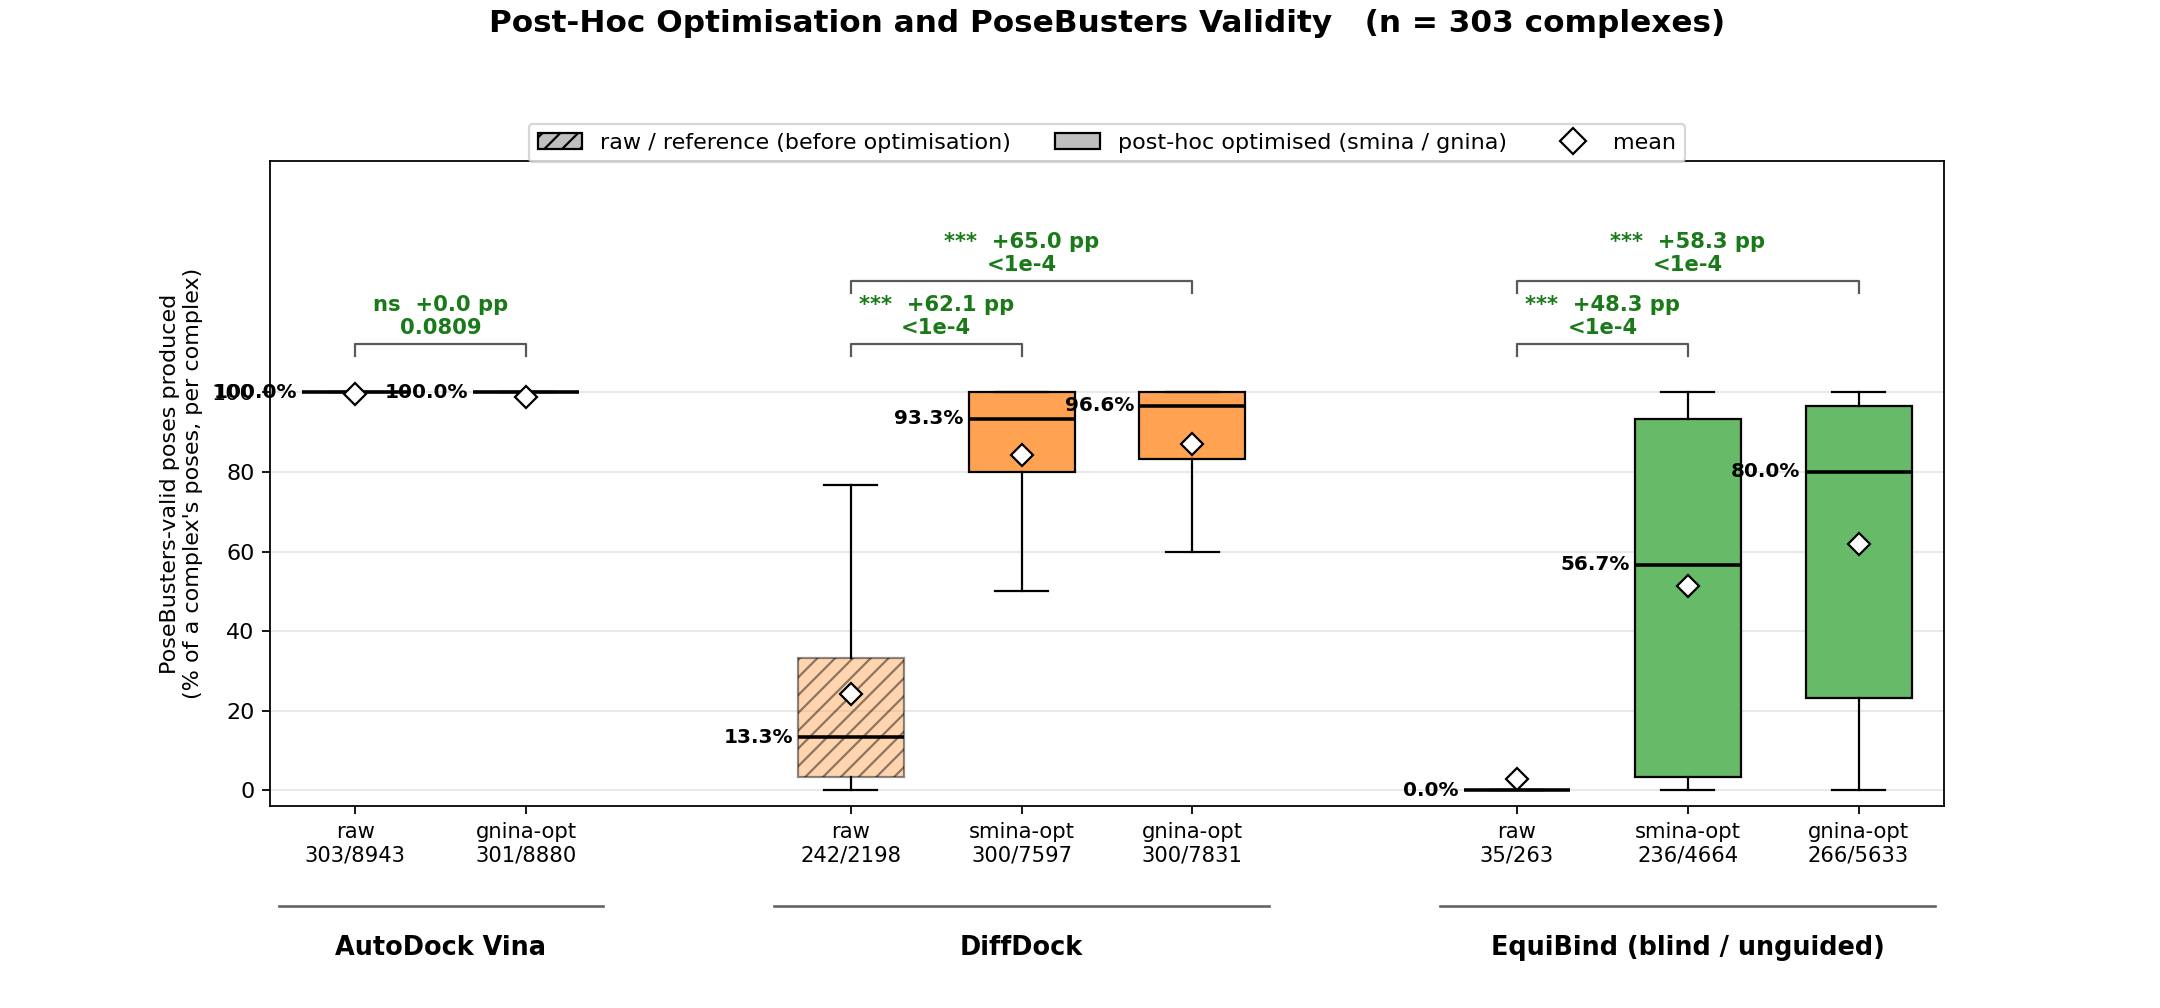
\includegraphics[width=\linewidth,height=0.78\textheight,keepaspectratio]{media/media/image2.png}
\caption{Post-hoc optimisation and PoseBusters validity. Significance brackets carry Holm-corrected p-values}\label{fig:results-r1}
\end{figure}

Figure~\ref{fig:results-r1} reports per-complex PoseBusters-validity yields before and after local optimisation. AutoDock's raw search is already almost perfectly valid. The median per-complex yield is 100\%, pooled validity is 99.6\%, and every one of the 303 complexes has at least one valid pose. Only 33 of 8,976 raw poses fail PoseBusters checks, split across internal clash (12), minimum distance to protein (20) and internal energy (1). Gnina rescoring leaves the median at 100\% and moves pooled validity to 98.9\%. The Hodges-Lehmann difference is exactly zero percentage points because 293 of the 303 complexes are unchanged, and the small movement that exists runs against rescoring (Wilcoxon p = 0.081). The two arms are level on physical validity with no headroom for an optimiser to repair.
DiffDock rises from a 13.3\% raw median to 93.3\% with smina, a Hodges-Lehmann gain of +62.1 percentage points. Unguided EquiBind rises from 0\% to 80.0\% with gnina. These near-unanimous gains survive Holm correction, with matched-pairs rank-biserial effects of 0.994--1.000 and adjusted p-values below 10\textsuperscript{-35}. DiffDock behaves similarly with gnina (96.6\%), whereas EquiBind performs worse with smina (56.7\%). The refiners are thus nearly interchangeable for DiffDock, while gnina is decisive for EquiBind.

% Removes since not relevant to the current discussion of PoseBusters validity.
% The hydrogen-handling artefact that inflates a raw-against-rescored validity comparison elsewhere does not arise here. Poses from the ADFRsuite-prepared arm carry no embedded SMILES, so both the raw and the rescored pose are rebuilt from a bond-order template as a heavy-atom record and PoseBusters adds and relaxes the whole hydrogen shell itself on each side. The added-hydrogen flag is set on 100\% of raw and 99.7\% of rescored poses, so the two arms are measured on the same footing and the comparison is a like-for-like one. What small movement there is runs against rescoring rather than for it, and it is concentrated rather than distributed. Rescoring raises internal-energy failures from 1 pose to 70 and leaves the intermolecular checks essentially unchanged, and 60 of the 63 additional invalid poses come from two complexes, 7NUT\_GLP and 7OZC\_G6S, which lose all thirty poses having been fully valid raw. The remaining 301 complexes still hold a valid rescored pose. Rescoring is therefore adopted for what it does to ranking, not to geometry, and the near-nativeness results below are where it earns its place. By contrast, minimisation makes most learned output physically valid.

Table~\ref{tab:appendix-pb-decomposition-full} in Appendix~\ref{supplementary-statistics} decomposes PoseBusters failure rates into the three groups. None of 72,219 poses from the eight reported variants fails a chemical-validity check. While only 25 poses fail bond length and 22 bond angle, most discrimination is intermolecular. Raw DiffDock has a 75.2\% intermolecular-failure rate against 75.6\% invalid overall, and raw EquiBind 96.8\% against 97.1\%. Minimum distance to protein dominates, failing 73.8\% of raw DiffDock and 96.5\% of raw EquiBind poses, compared with 0.2\% for AutoDock. Intramolecular failures matter only for raw EquiBind (27.9\%, versus at most 3.8\% for any AutoDock or DiffDock variant). A Benjamini-Hochberg analysis of the sixteen varying checks retains thirteen at q \textless{} 0.05, with minimum distance strongest (cp. Appendix~\ref{supplementary-statistics} for full analysis). Conditioning on poses already within 2\angstrom{} of the crystal indicates that placement, not chemistry, explains most of the remaining gap. The validity requirement removes at most four of 303 complexes from the headline endpoint at any depth. Appendix~\ref{validity-objective-coupling} reports both quantities and the overlap between intermolecular checks and the coordinate optimised by the search objective.

Table~\ref{tab:results-depth-recovery} compares rank-1, best-of-top-15 and best-of-top-30 pools. A complex is recovered if any inspected pose is PoseBusters-valid and within 2\angstrom{}. Because these pools are nested, deeper inspection can only add recoveries. All discordant pairs within a depth step therefore point in one direction, making recovery shares and confidence intervals more informative than a two-directional test. That test retains its usual interpretation between tools. Appendix~\ref{supplementary-statistics} gives the procedure.

\begin{longtable}[]{@{}
  >{\raggedright\arraybackslash}p{(\columnwidth - 10\tabcolsep) * \real{0.1156}}
  >{\raggedleft\arraybackslash}p{(\columnwidth - 10\tabcolsep) * \real{0.1573}}
  >{\raggedleft\arraybackslash}p{(\columnwidth - 10\tabcolsep) * \real{0.1573}}
  >{\raggedleft\arraybackslash}p{(\columnwidth - 10\tabcolsep) * \real{0.1573}}
  >{\raggedleft\arraybackslash}p{(\columnwidth - 10\tabcolsep) * \real{0.2059}}
  >{\raggedleft\arraybackslash}p{(\columnwidth - 10\tabcolsep) * \real{0.2065}}@{}}
\caption{PoseBusters Pass-All Recovery by Ranking Depth}\label{tab:results-depth-recovery}\tabularnewline
\toprule\noalign{}
{\raggedright \textbf{Method}} & \centering\arraybackslash\textbf{Rank-1} & \centering\arraybackslash\textbf{Best of top-15} & \centering\arraybackslash\textbf{Best of top-30} & \centering\arraybackslash\textbf{top-1\ensuremath{\rightarrow}15 gain} & \centering\arraybackslash\textbf{top-15\ensuremath{\rightarrow}30 gain} \\
\midrule\noalign{}
\endfirsthead
\caption[]{PoseBusters Pass-All Recovery by Ranking Depth (continued)}\tabularnewline
\toprule\noalign{}
{\raggedright \textbf{Method}} & \centering\arraybackslash\textbf{Rank-1} & \centering\arraybackslash\textbf{Best of top-15} & \centering\arraybackslash\textbf{Best of top-30} & \centering\arraybackslash\textbf{top-1\ensuremath{\rightarrow}15 gain} & \centering\arraybackslash\textbf{top-15\ensuremath{\rightarrow}30 gain} \\
\midrule\noalign{}
\endhead
\bottomrule\noalign{}
\endlastfoot
{\raggedright AutoDock} & {\raggedright 36.6\% (111)} & {\raggedright 65.3\% (198)} & {\raggedright 65.7\% (199)} & {\raggedright +87 (+28.7\%) ***} & {\raggedright +1 (+0.3\%)} \\
DiffDock & 34.0\% (103) & 55.1\% (167) & 55.8\% (169) & +64 (+21.1\%) *** & +2 (+0.7\%) \\
EquiBind & 18.2\% (55) & 26.4\% (80) & 26.4\% (80) & +25 (+8.3\%) *** & +0 (+0.0\%) \\
\multicolumn{6}{@{}p{\dimexpr\columnwidth-6\tabcolsep\relax}@{}}{\footnotesize%
Two-sided McNemar tests with Holm-Bonferroni correction, *** p \textless{} 0.001, ** p \textless{} 0.01 and * p \textless{} 0.05} \\
\multicolumn{6}{@{}p{\dimexpr\columnwidth-6\tabcolsep\relax}@{}}{\footnotesize%
Recovery is the PoseBusters-valid, within-2\angstrom{} recovery also reported across distance thresholds in Table~\ref{tab:results-near-native-form}, and the two coincide at every depth shown here.} \\
\end{longtable}
% UPDATED 2026-08-29 for the MGLTools/ADFRsuite exh128 arm; same existence gate as before
% (any pose in top-d that is PB-valid AND RMSD<=2A). Counts from
% benchmark_matched_equibind/.../per_pose_metrics.csv, DOMINANT AutoDock arm
% (REPOINTED 2026-09-01 from the superseded benchmark_full_protein_vina_scoring tree.)
% autodock_mgltools_exh128_gnina: 111/198/199 (the raw exh128 arm is 94/185/202 and must NOT be
% used to regenerate this table). Superseded Meeko figures were 89/151/151.
% OLD NOTE, kept for provenance:
% DiffDock-smina 103/167/169, EquiBind-gnina 55/80/80 (--minimize arm, re-derived 2026-09-01;
% the superseded --local_only arm read 46/61/62 and must NOT be used).
% Depth-gain decomposition (appendix tab:results-depth-gain), same gnina/smina arm, re-derived
% 2026-09-01 from benchmark_matched_equibind: near-native gained +88/+63/+26; of which remain
% PB-invalid -2/-1/-2; valid rescued +1/+2/+1; net +87/+64/+25, matching this table's gain column.
% 15->30 gains on the PRINTED gnina/smina arm (autodock_gnina by optimized_rank, diffdock_smina,
% equibind_unguided_gnina by gnina_affinity): discordant b = 0/2/1, c = 0 throughout, exact two-sided
% p = 1.0/0.5/1.0, none significant (no stars). Counts 198->199, 167->169, 80->80,
% discordant b = 1/2/0, c = 0 throughout (re-derived 2026-09-01 on the --minimize arm).
% (An earlier note here recorded b=5 -> p=0.0625; that is the RAW Vina arm 145->150, which the lines
%  above forbid for this table. Re-derived 2026-08-16 from per_pose_metrics.csv.)

Table~\ref{tab:results-depth-gain} in Appendix~\ref{supplementary-statistics} decomposes the reservoir of lower-ranked PoseBusters-valid poses in greater detail. 


\hypertarget{near-nativeness-and-form}{%
\subsection{Near-Nativeness and Form}\label{near-nativeness-and-form}}

Figures~\ref{fig:results-r2a} and \ref{fig:results-r2b} report accuracy for the 303 complexes with PoseBusters-valid poses against as-placed crystal RMSD (i.e. near-nativeness) and best-fit Kabsch RMSD (i.e. form), separating placement from form. The vertical axis gives the percentage of complexes with at least one valid pose within the distance threshold among the first d ranks. Differences among the top-1, top-15 and top-30 curves measure ranking headroom \footnote{Table~\ref{tab:results-near-native-form} in Appendix~\ref{supplementary-statistics} provides ten distance thresholds.}, namely valid near-native poses generated but ranked below d, distinguishing sampling from scoring \cite{ref050}, \cite{ref052}. 

Near-native recovery differs among tools at every depth (Cochran\textquotesingle s Q p \textless{} 1e-7). At 2\angstrom{}, AutoDock has the highest point estimate with margins over DiffDock opening at top-5 and narrowing slightly with increasing depth. Rank-1 accuracy is 36.6\% for AutoDock, 34.0\% for DiffDock and 18.2\% for EquiBind. AutoDock and DiffDock exceed EquiBind at every depth (all p\_holm \textless{} 3e-7). AutoDock and DiffDock do not differ detectably at rank-1, where the gap is +2.6 percentage points (Newcombe hybrid-score 95\% interval \ensuremath{-}4.2 to +9.4, exact McNemar p = 0.509), but they do from top-5 onwards, by +13.2 points at top-5 (+5.7 to +20.4, p\_holm = 7.6e-4), +10.2 at top-15 (+2.8 to +17.5, p\_holm = 0.009) and +9.9 at top-30 (+2.5 to +17.1, p\_holm = 0.011). Thus, ordering is a statement about the pool inspected rather than about a single nominated pose, where the two tools remain indistinguishable. 

However, AutoDock's lead is attributed to fine-tuning exhaustiveness (cp. Appendix~\ref{exhaustiveness-selection}) whereas DiffDock and EquiBind arms enhancement was based on post-hoc refinement solely. The head-to-head comparison sets a tuned pipeline against two untuned ones, and the AutoDock figures carry a rank-1 selection optimism that the other two do not, quantified in the same appendix. What the ordering establishes is narrower than a comparison of method classes. The carried-forward AutoDock arm is itself CNN-rescored by gnina. The contrast is therefore between two configured workflows on this benchmark and not between physics-based and AI-based docking.

The rank-1 contrast draws information only from the 112 discordant complexes, so the minimum detectable difference there is 9.8 percentage points at 80\% power and the study is underpowered for the observed +2.6-point estimate. No equivalence margin was prespecified, and the non-significant rank-1 result does not establish equivalence. Appendix~\ref{supplementary-statistics} gives the power calculation and projected sample size.

Ranking depth affects every tool (Cochran\textquotesingle s Q p \textless{} 1e-6 throughout). From rank-1 to best-of-top-15, AutoDock gains +28.7 percentage points (Wilson 95\% interval 23.9--34.0), DiffDock +21.1 (16.9--26.1) and EquiBind +8.3 (5.7--11.9). AutoDock rises from 36.6\% to 65.3\%, adding 87 complexes compared with DiffDock\textquotesingle s 64. The selection gaps align with the sampling and scoring distinction \cite{ref003}, \cite{ref050}, \cite{ref052} and with the gap DiffDock reports between its top-ranked pose and its wider sample \cite{ref024}. Rescoring with gnina captures part of that headroom prospectively rather than retrospectively, raising AutoDock\textquotesingle s rank-1 recovery from 31.0\% to 36.6\% and its top-15 recovery from 61.1\% to 65.3\%. Since that pass reorders the pool rather than enlarging it, the gain is confined to the top of the list. Over the whole pool the raw search is nominally ahead, 202 complexes against 199, because rescoring minimises every pose and a few cross the threshold the wrong way (Appendix~\ref{exhaustiveness-selection}). EquiBind\textquotesingle s smaller gain indicates a sampling constraint. A single-shot regression model provides few distinct alternatives, and rescoring cannot recover poses that were not generated.

\begin{figure}[!htbp]
\centering
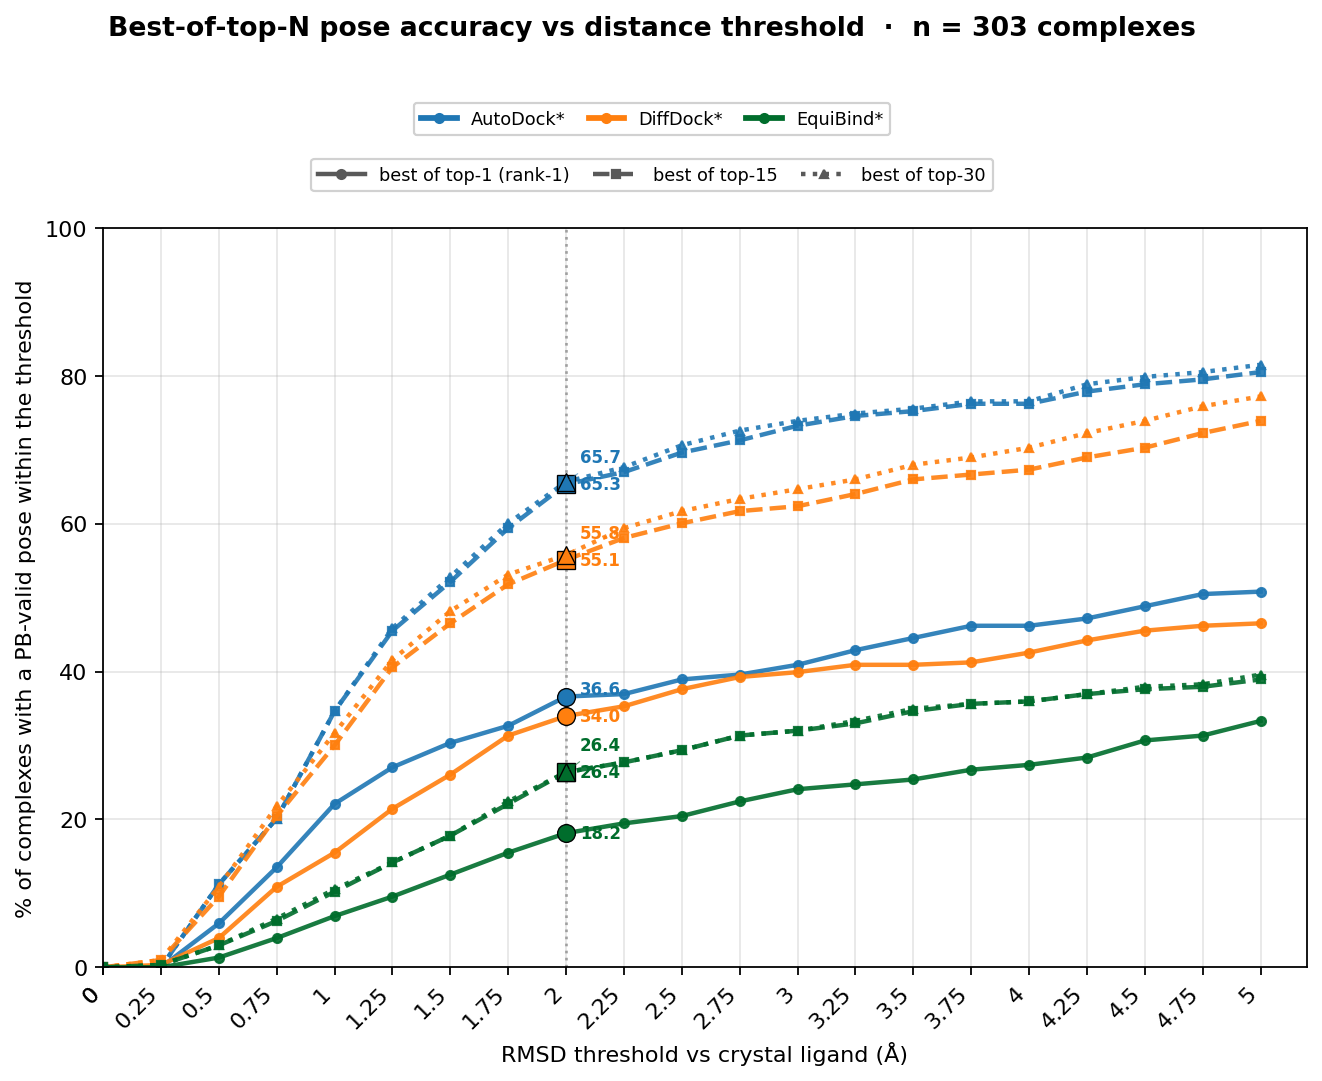
\includegraphics[width=0.86\linewidth,height=0.78\textheight,keepaspectratio]{media/media/image3.png}
\caption{Best-of-top-N accuracy against the as-placed crystal RMSD}\label{fig:results-r2a}
\end{figure}

Kabsch RMSD isolates ligand form. AutoDock and DiffDock recover 74.3\% and 74.6\%, respectively, at the primary 1\angstrom{} threshold and best-of-top-30 depth, compared with 95.4\% and 97.0\% at 2\angstrom{}. Form differs among tools at every depth (Cochran\textquotesingle s Q p \textless{} 1e-9). Rank-1 recovery is 52.5\% for AutoDock, 52.1\% for DiffDock and 33.3\% for EquiBind. AutoDock and DiffDock exceed EquiBind at every depth (p\_holm \ensuremath{\leq} 4e-10). In contrast, the AutoDock--DiffDock comparison is a tie throughout, at p\_holm = 1.000 with 47 against 46 discordant complexes at rank-1, 30 against 31 at top-15 and 25 against 26 at top-30. Form is the one axis on which a physics-based search and a diffusion model are statistically indistinguishable. No equivalence margin was prespecified. This is an absence of detected difference rather than a demonstration of equivalence. DiffDock generates the right shape and localises it less well, consistent with its generative treatment of torsional, rotational and translational degrees of freedom \cite{ref024}. AutoDock samples rigid-receptor placements whose internal geometry is constrained by construction.

\begin{figure}[!htbp]
\centering

\includegraphics[width=0.86\linewidth,height=0.78\textheight,keepaspectratio]{media/media/image4.png}
\caption{Best-of-top-N accuracy against the best-fit (Kabsch) RMSD}\label{fig:results-r2b}
\end{figure}

EquiBind remains weakest on form, rising from 33.3\% at rank-1 to 54.1\% at best-of-top-30. This indicates internal-geometry error in addition to misplacement and agrees with evaluations in which direct regression trails diffusion and hybrid methods on combined geometry and validity \cite{ref013}, \cite{ref035}. The 20.8-point depth gain provides evidence of acceptable but mislocated shape poses. From top-15 to top-30, placement gains at most 0.7 points, whereas form at 1\angstrom{} gains 2.3 points for both AutoDock and DiffDock and 3.0 for EquiBind (Table~\ref{tab:results-near-native-form}).

The near-nativeness and form endpoints separate the tools differently. On placement AutoDock leads from top-5 onwards. On form AutoDock and DiffDock are indistinguishable everywhere. On pooled physical validity AutoDock leads throughout, at 98.9\% against 84.5\% for DiffDock. Their top-15 selection gains are 87 and 64 complexes, yet about six in ten rank-1 failures contain no qualifying pose anywhere in the pool. Generation and localisation therefore remain the larger constraints \cite{ref003}, \cite{ref013}, \cite{ref024}, \cite{ref035}. Refined-score ordering can be considered an unclaimed remedy for DiffDock, worth about three points of rank-1 recovery on the reported coordinates. For AutoDock a larger sampling budget was tested directly (cp. Appendix~\ref{exhaustiveness-selection}).

Figure~\ref{fig:results-r3} plots in-place against Kabsch RMSD, separating placement-limited, form-limited and mixed errors. Its columns expand the pool from rank-1 to best-of-top-5 and best-of-top-15. Arrows trace each cohort median from rank-1. Table~\ref{tab:results-placement-form} in Appendix~\ref{supplementary-statistics} provides details about the distributions.\footnote{Poses whose docked centroid lies more than 8\angstrom{} from the crystal-ligand site were removed leaving 6,169 PoseBusters-valid poses for scoring. Axes are clipped at 5\angstrom{} keeping dense near-native core legible, yet removing 2,329 poses from the graph frame.}

AutoDock returns a valid pose for all 303 complexes, but only 62.7\% remain after the rank-1 crystal-site trim. Its median in-place RMSD deteriorates most with depth, from 1.5\angstrom{} at rank-1 to 5.0\angstrom{} at top-15. The +3.55\angstrom{} shift has a receptor-bootstrap interval of +3.00 to +3.99\angstrom{} and is supported across disjoint within-complex rank bands (Friedman p \textless{} 1e-15). Placement-limited poses rise from 48\% to 78\%, while form-limited poses fall from 27\% to 8\%. Deeper ranks therefore add mainly correctly shaped but misplaced ligands, consistent with the largest within-complex spread (5.72\angstrom{}). Ranking is informative only near the top.

DiffDock is most stable with depth in the near-site cohort, drifting +0.46\angstrom{} in place versus +3.55\angstrom{} for AutoDock and +1.09\angstrom{} for EquiBind. Expanding the pool fifteen-fold keeps DiffDock medians near 1.5--1.9\angstrom{} in place and 0.9\angstrom{} in form. It is significantly best on both axes at top-5 and top-15. Form shifts only +0.03\angstrom{} (bootstrap interval \ensuremath{-}0.05 to +0.12\angstrom{}), although disjoint rank bands differ across the 137 complete complexes (Friedman p = 0.006). This statistically detected but negligible change partly reflects low diversity. DiffDock\textquotesingle s within-complex spread is 2.34\angstrom{}, compared with 5.72\angstrom{} for AutoDock.

EquiBind produces at least one valid pose for 266 of 303 complexes, but valid-near-native recovery is only 26.4\% by top-15 and 26.4\% over all thirty poses. Its rank-1 median in-place RMSD of 2.9\angstrom{} already exceeds the near-native threshold. Gnina minimisation repairs some local defects but not gross localisation failures.

\begin{figure}[!htbp]
\centering

\includegraphics[width=0.86\linewidth,height=0.78\textheight,keepaspectratio]{media/media/image5.png}
\caption{Form versus in-place RMSD across ranking depth}\label{fig:results-r3}
\end{figure}

In the near-site cohort, deeper ranks add valid but misplaced AutoDock and EquiBind poses and few for DiffDock. In-place RMSD deteriorates with depth. DiffDock appears more form-limited only because its low in-place RMSD inflates the form-to-in-place ratio. Its absolute form RMSD is lowest.

\hypertarget{cross-tool-clustering}{%
\subsection{Cross-Tool Clustering}\label{cross-tool-clustering}}

Poses from the three selected variants were pooled without validity filtering, clustered and scored for crystal-site recovery under the 4\angstrom{} rule defined in the Methods. Sixteen of 303 complexes have no qualifying cluster and count as non-reaches. Figure~\ref{fig:results-r4} and Table~\ref{tab:results-cluster-recovery} report top-N recovery for individual tools and combinations.

\begin{figure}[!htbp]
\centering

\includegraphics[width=\linewidth,height=0.78\textheight,keepaspectratio]{media/media/image6.png}
\caption{Top-N crystal-cluster co-recovery}\label{fig:results-r4}
\end{figure}

AutoDock and DiffDock have almost fully overlapping reach intervals at every depth, while EquiBind trails both. From rank-1 to top-15, DiffDock gains 26 percentage points, AutoDock 24 and EquiBind 4. Pairings become less redundant with depth but remain positively associated. At top-15, all converge at \ensuremath{\phi} = +0.23 to +0.28 with Fisher p \ensuremath{\leq} 2.8e-4.

\begin{longtable}[]{@{}
  >{\raggedright\arraybackslash}p{(\columnwidth - 8\tabcolsep) * \real{0.4200}}
  >{\centering\arraybackslash}p{(\columnwidth - 8\tabcolsep) * \real{0.1450}}
  >{\centering\arraybackslash}p{(\columnwidth - 8\tabcolsep) * \real{0.1450}}
  >{\centering\arraybackslash}p{(\columnwidth - 8\tabcolsep) * \real{0.1450}}
  >{\centering\arraybackslash}p{(\columnwidth - 8\tabcolsep) * \real{0.1450}}@{}}
\caption{Crystal-Cluster Reach and Co-Reach by Ranking Depth}\label{tab:results-cluster-recovery}\tabularnewline
\toprule\noalign{}
{\raggedright \textbf{Statistic}} & \centering\arraybackslash\textbf{top-1} & \centering\arraybackslash\textbf{top-5} & \centering\arraybackslash\textbf{top-10} & \centering\arraybackslash\textbf{top-15} \\
\midrule\noalign{}
\endfirsthead
\caption[]{Crystal-Cluster Reach and Co-Reach by Ranking Depth (continued)}\tabularnewline
\toprule\noalign{}
{\raggedright \textbf{Statistic}} & \centering\arraybackslash\textbf{top-1} & \centering\arraybackslash\textbf{top-5} & \centering\arraybackslash\textbf{top-10} & \centering\arraybackslash\textbf{top-15} \\
\midrule\noalign{}
\endhead
\bottomrule\noalign{}
\endlastfoot
AutoDock reach \% {[}95\% CI{]} & 59 {[}53--64{]} & 79 {[}74--83{]} & 81 {[}76--85{]} & 83 {[}79--87{]} \\
DiffDock reach \% {[}95\% CI{]} & 54 {[}49--60{]} & 76 {[}70--80{]} & 79 {[}74--83{]} & 81 {[}76--85{]} \\
EquiBind reach \% {[}95\% CI{]} & 43 {[}37--49{]} & 46 {[}40--51{]} & 47 {[}41--52{]} & 47 {[}42--53{]} \\
AutoDock + DiffDock co-reach\footnote{Co-reach \ensuremath{\phi} is the signed association between two tools\textquotesingle{} per-complex reach against independence, where a positive value means the pair succeeds and fails together. All three pairings reach p \textless{} 0.05 on a two-sided Fisher test. Three-way agreement exceeds chance at every depth with a permutation p below 1e-4, and the ranking depths are nested cumulative thresholds rather than an independent test family.} \ensuremath{\phi} & \textbf{+0.33} & \textbf{+0.23} & \textbf{+0.24} & \textbf{+0.23} \\
AutoDock + EquiBind co-reach \ensuremath{\phi} & \textbf{+0.45} & \textbf{+0.27} & \textbf{+0.29} & \textbf{+0.28} \\
DiffDock + EquiBind co-reach \ensuremath{\phi} & \textbf{+0.42} & \textbf{+0.30} & \textbf{+0.29} & \textbf{+0.26} \\
All three reach, complexes observed / expected & 89 / 42 & 114 / 82 & 121 / 90 & 125 / 96 \\
\multicolumn{5}{@{}p{\dimexpr\columnwidth-5\tabcolsep\relax}@{}}{\footnotesize%
The three reach rows are percentages of the 303 complexes, carried with Wilson 95\% intervals.} \\
\end{longtable}

\begin{figure}[!htbp]
\centering
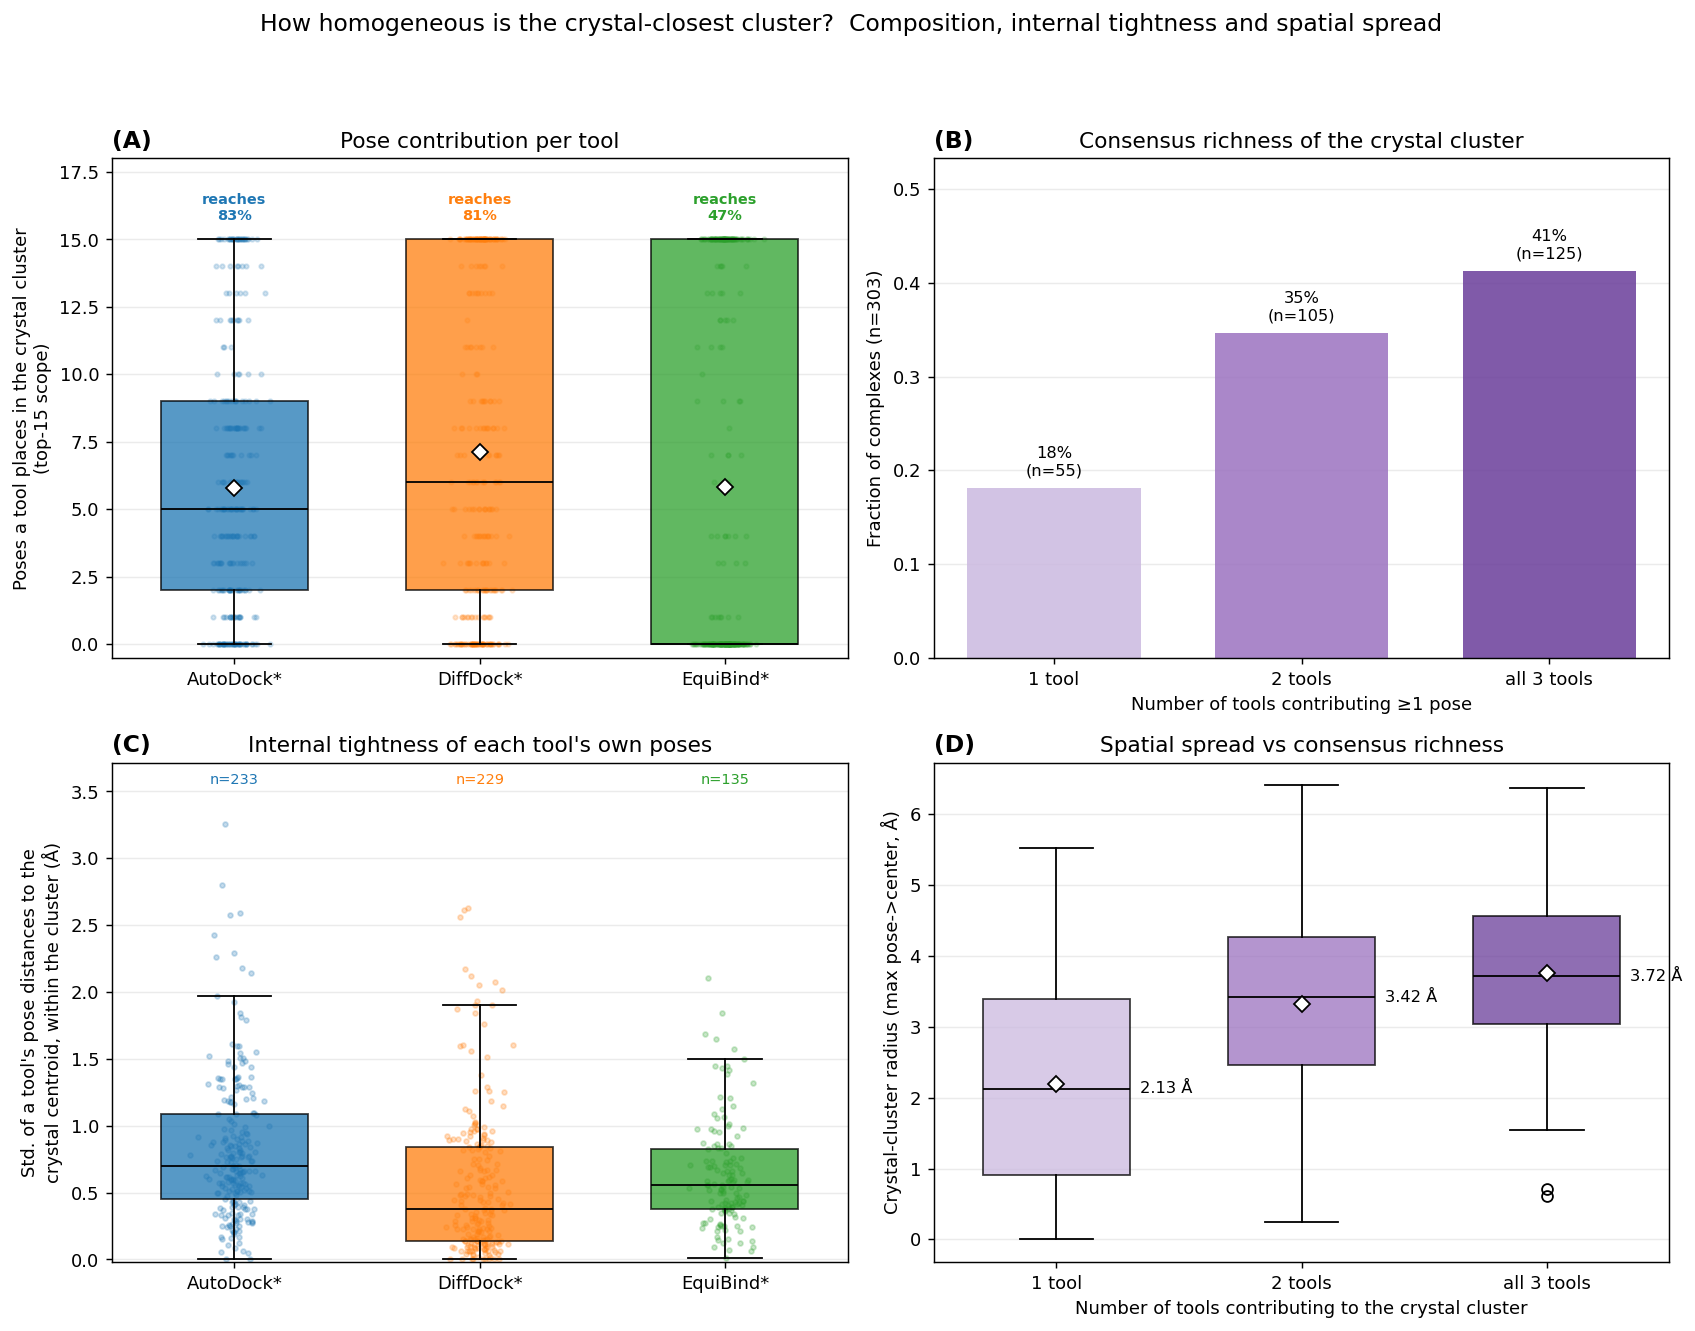
\includegraphics[width=\linewidth,height=0.78\textheight,keepaspectratio]{media/media/image7.png}
\caption{Composition and geometry of the crystal-closest cluster. Rates are taken over all 303 complexes, 18 of which contribute no pose to any panel}\label{fig:results-r5}
\end{figure}

Figure~\ref{fig:results-r5} (A) gives DiffDock a median six of fifteen poses in the crystal cluster and 81\% reach, and AutoDock five poses and 83\% reach. EquiBind has a median of zero and 47\% reach. In the reported top-15 analysis the two leading tools differ in pose count, where DiffDock contributes more (Holm-corrected rank-biserial \ensuremath{-}0.28, p = 2.7e-4), but not in reach (McNemar p = 0.470 on 38 against 31 discordant complexes). Both exceed EquiBind on reach. Panel (B) shows polarised consensus, with 125 complexes solved by all tools versus 96.1 expected (permutation p \textless{} 1e-4), and 18 by none versus 5.2 expected. AutoDock accounts for 28 of the 55 single-tool solutions, compared with 25 for DiffDock and two for EquiBind. Panel (C) plots, for each complex and tool, the standard deviation of that tool\textquotesingle s in-cluster poses in their distance to the crystal centroid. The median is 0.70\angstrom{} for AutoDock over 233 defined complexes, 0.56\angstrom{} for EquiBind over 135 and 0.38\angstrom{} for DiffDock over 229. Cohorts differ because the statistic requires at least two within-cluster poses, making missingness informative. The measure is radial, and poses lying at a common distance from the crystal centroid can still sit far apart. A large value therefore establishes real spatial spread, whereas a small value does not establish that a tool\textquotesingle s poses sit together. The supported reading is that AutoDock scatters its in-cluster poses along the radial coordinate. A paired restriction to the 110 complexes defined for all tools keeps AutoDock highest on this statistic, at 0.70\angstrom{} against 0.57\angstrom{} and 0.31\angstrom{}. Appendix~\ref{supplementary-statistics} gives the omnibus and pairwise statistics.

Panel (D) shows median cluster radius increasing from 2.13\angstrom{} for single-tool clusters to 3.72\angstrom{} for three-tool clusters, but the association is no longer detectable after adjustment for pose count (partial \ensuremath{\rho} = \ensuremath{-}0.07, p = 0.26). The partition has a median bootstrap Jaccard of 0.78. At the 4\angstrom{} crystal-site threshold, the retrospective oracle recovers 95\% of complexes, compared with about 56\% for the best inexpensive first-cluster rules. Consensus ranking reaches 56.8\%, its medoid-centred variant 55.4\% and confidence weighting 55.8\%. These three rules are not separable from one another, and they gain 7.3, 5.9 and 6.3 points respectively on the 49.5\% legacy pose-count rule. All three clear correction against it (Holm-corrected McNemar p = 3.6e-4 for consensus ranking, 0.004 for confidence weighting and 0.008 for its medoid-centred variant). The 38-point oracle gap reflects site ranking. The pooled cloud usually contains the crystal-compatible region, but blind prospective selection remains difficult. Figure~\ref{fig:results-r6} in Appendix~\ref{supplementary-statistics} reports internal validity, resampling stability and precision-at-one for all five rules.

Across the full pose cloud, the pooled three-tool oracle places a pose within 4\angstrom{} of the crystal site for 97.7\% of complexes, at a median distance of 0.34\angstrom{}. AutoDock alone reaches 88.1\% at 0.53\angstrom{} and DiffDock 84.5\% at 0.56\angstrom{}. Together they already reach 97.7\% at 0.37\angstrom{}, so EquiBind adds nothing to the pooled reach. Averaging cluster members makes the pooled centre coarser than the best individual pose, with a median distance of 1.23\angstrom{}.

\hypertarget{interaction-and-contact-analysis}{%
\subsection{Interaction and Contact Analysis}\label{interaction-and-contact-analysis}}

Crystal-pose interactions are compared with those of PoseBusters-valid pipeline poses. PandaMap detects typed contacts \cite{ref090} using PLIP-style categories \cite{ref054} but only distance and atom-type criteria in this execution path. Because fingerprints encode residue identity, all poses and the crystal reference use one common author-numbered receptor per complex (Appendix~\ref{interaction-fingerprints}). Figure~\ref{fig:results-r7} gives mean Jaccard overlap for each tool\textquotesingle s top-5 union. Each cell averages the complexes for which both entries are defined, not one matrix-wide cohort.

\begin{figure}[!htbp]
\centering

\includegraphics[width=\linewidth,height=0.78\textheight,keepaspectratio]{media/media/image9.png}
\caption{Mean Jaccard similarity of interaction fingerprints, whole-protein search}\label{fig:results-r7}
\end{figure}

DiffDock has the highest mean typed-interaction Jaccard similarity to the crystal, at 0.450 over 300 complexes, compared with 0.417 over 301 for AutoDock and 0.380 over 266 for EquiBind. That ordering survives restriction to a common cohort. Across the 264 complexes defined for all tools, DiffDock reaches 0.474, AutoDock 0.431 and EquiBind 0.381. DiffDock leads AutoDock (Wilcoxon p = 0.014) and both exceed EquiBind (p = 1.6e-3 and 5.2e-8). AutoDock averages only 0.313 on the 37 complexes lacking a valid EquiBind pose. Pairwise tool similarities range from 0.357 to 0.463, and the AutoDock--DiffDock pair at 0.463 exceeds either tool\textquotesingle s similarity to the crystal. The two therefore resemble each other more than either resembles the reference and thus have different contact hypotheses. Because Jaccard counts both shared and non-shared interactions, it is not contact recall.

Table~\ref{tab:results-native-recovery-rank} reports precision, recall and F1 by each tool\textquotesingle s own rank k among all produced poses, profiling only PoseBusters-valid poses. AutoDock uses gnina re-ranking, EquiBind gnina affinity and DiffDock native confidence retained through smina refinement. A failed top-ranked pose contributes no k = 1 value, affecting 5 of 303 AutoDock complexes and 21 of the 303 with DiffDock output. EquiBind ranks only retained valid poses and therefore always begins at k = 1.

Rank-1 F1 is 0.57 for AutoDock, 0.53 for DiffDock and 0.47 for EquiBind, but these means use different available-case cohorts and were not tested for equivalence. Across 280 shared AutoDock--DiffDock complexes, the means are 0.5663 and 0.5324 without a detected difference (Wilcoxon p = 0.25). Scoring a missing valid rank-1 pose as zero across all 303 complexes preserves the order and widens it, to 0.556 for AutoDock and 0.492 for DiffDock, which more often lacks a valid nominee. Rank-1 contact fidelity is therefore conditional on a valid top pose, though the ordering here is not sensitive to how missing poses are treated. By rank 5, AutoDock declines to 0.42, while DiffDock remains near 0.51 and EquiBind near 0.44. DiffDock consequently leads for the top-5 union in Figure~\ref{fig:results-r7} without leading on the nominated pose. Per-complex Kendall \ensuremath{\tau} links AutoDock rank to better poses. EquiBind gnina-affinity rank similarly orders recall and F1. DiffDock confidence has no detected association with interaction recovery, so its top pose cannot be expected from these data to outperform rank 5. This is absence of detected ordering, not proof that confidence lacks signal. Appendix~\ref{supplementary-statistics} gives the nine BH-corrected \ensuremath{\tau} tests.

\begin{longtable}[]{@{}
  >{\raggedright\arraybackslash}p{(\columnwidth - 10\tabcolsep) * \real{0.3000}}
  >{\centering\arraybackslash}p{(\columnwidth - 10\tabcolsep) * \real{0.1400}}
  >{\centering\arraybackslash}p{(\columnwidth - 10\tabcolsep) * \real{0.1400}}
  >{\centering\arraybackslash}p{(\columnwidth - 10\tabcolsep) * \real{0.1400}}
  >{\centering\arraybackslash}p{(\columnwidth - 10\tabcolsep) * \real{0.1400}}
  >{\centering\arraybackslash}p{(\columnwidth - 10\tabcolsep) * \real{0.1400}}@{}}
\caption{Native-Interaction Recovery versus the Crystal by Pose Rank, Whole-Protein Search}\label{tab:results-native-recovery-rank}\tabularnewline
\toprule\noalign{}
{\raggedright \textbf{Tool and statistic}} & \centering\arraybackslash\textbf{k = 1} & \centering\arraybackslash\textbf{k = 2} & \centering\arraybackslash\textbf{k = 3} & \centering\arraybackslash\textbf{k = 4} & \centering\arraybackslash\textbf{k = 5} \\
\midrule\noalign{}
\endfirsthead
\caption[]{Native-Interaction Recovery versus the Crystal by Pose Rank, Whole-Protein Search (continued)}\tabularnewline
\toprule\noalign{}
{\raggedright \textbf{Tool and statistic}} & \centering\arraybackslash\textbf{k = 1} & \centering\arraybackslash\textbf{k = 2} & \centering\arraybackslash\textbf{k = 3} & \centering\arraybackslash\textbf{k = 4} & \centering\arraybackslash\textbf{k = 5} \\
\midrule\noalign{}
\endhead
\bottomrule\noalign{}
\endlastfoot
AutoDock complexes n & 298 & 298 & 299 & 296 & 299 \\
AutoDock precision & 0.561 & 0.550 & 0.485 & 0.497 & 0.439 \\
AutoDock recall & 0.572 & 0.548 & 0.477 & 0.479 & 0.414 \\
AutoDock F1 & 0.565 & 0.546 & 0.479 & 0.485 & 0.423 \\
DiffDock complexes n & 282 & 267 & 277 & 270 & 275 \\
DiffDock precision & 0.536 & 0.529 & 0.520 & 0.497 & 0.528 \\
DiffDock recall & 0.526 & 0.511 & 0.496 & 0.471 & 0.504 \\
DiffDock F1 & 0.529 & 0.517 & 0.503 & 0.479 & 0.512 \\
EquiBind complexes n & 266 & 256 & 247 & 245 & 243 \\
EquiBind precision & 0.493 & 0.489 & 0.488 & 0.476 & 0.472 \\
EquiBind recall & 0.459 & 0.451 & 0.450 & 0.433 & 0.423 \\
EquiBind F1 & 0.471 & 0.465 & 0.463 & 0.449 & 0.441 \\
\multicolumn{6}{@{}p{\dimexpr\columnwidth-6\tabcolsep\relax}@{}}{\footnotesize%
Each cell is the unweighted mean over the complexes that contribute a PoseBusters-valid pose at that rank. The three tools are therefore compared on overlapping rather than identical cohorts.} \\
\end{longtable}

Figure~\ref{fig:results-r9} in Appendix~\ref{supplementary-statistics} decomposes these poses into matched, missed and spurious contacts. At rank 1, AutoDock and DiffDock recover 21.0 and 19.4 native contacts while missing 15.3 and 16.4. By rank 5, AutoDock falls to 15.3 matched against 21.0 missed, while spurious contacts rise to 17.6. It is the only pipeline whose spurious count increases significantly with rank. DiffDock remains near 18.6 matched and 17.4 missed with stable spurious counts. EquiBind misses more native contacts than it recovers at every rank, under-reproducing the native network while generating the fewest non-native contacts.

AutoDock and DiffDock show no detected difference in nominated rank-1 contact fidelity, but the result is inconclusive rather than equivalent. Gnina ranks AutoDock\textquotesingle s steeply declining series informatively, with all three per-complex Kendall correlations negative and surviving correction. DiffDock\textquotesingle s flatter pool remains unordered, and neither tested refined score improves it. EquiBind recovers few native contacts at any rank.

\protect\hypertarget{_Toc235735934}{}{}

\hypertarget{experimental-dataset-1}{%
\section{Experimental Dataset}\label{experimental-dataset-1}}

The experimental evaluation tests whether the ordering established against crystallographic references transfers to a pharmacologically relevant target. The Orai1 channel was docked with three functionally validated modulators, 2-APB, GSK-7975A and Synta-66. No ligand-bound Orai structure exists, and the receptor is an ensemble of molecular-dynamics snapshots. The Appendix (Docking Protocols, Orai1 Panels) specifies the settings and differences between the panels.

The experimental panel pairs three modulators with four Orai1 frames, providing twelve frame-ligand units. The control panel adapts the decoy-set practice of docking a large library of molecules, i.e. calibration dataset ligands, with no known target activity \cite{ref045}, \cite{ref046}, against which the compounds of interest are compared. The control panel is only a background comparator, and no enrichment claim is made. Of 1,232 possible combinations of 308 calibration ligands and four frames, AutoDock and EquiBind cover all 1,232 while DiffDock covers 1,215, i.e. the cross-tool comparisons rest on 1,215 units. Both panels use the selected calibration variant of each engine, namely AutoDock Vina + gnina, DiffDock + smina and EquiBind + gnina. Output is capped at the top ten ranked poses per unit, or the top three for interaction and contact analysis. DiffDock returned fewer than ten poses for 178 of its 1,215 units. Per-unit rates therefore use the poses produced, not a fixed denominator of ten. Appendix~\ref{orai1-panels} gives the per-frame drops and panel totals. Poses within a unit are correlated, and the twelve experimental units represent only three chemotypes and one receptor trajectory. Comparisons are therefore exploratory and emphasise effect sizes and uncertainty rather than p-values alone.

Table~\ref{tab:results-orai-yield} provides the end-to-end yield funnel, from produced poses through PoseBusters validity to the combined validity-and-placement endpoint.

\begin{longtable}[]{@{}
  >{\raggedright\arraybackslash}p{(\columnwidth - 12\tabcolsep) * \real{0.2140}}
  >{\raggedright\arraybackslash}p{(\columnwidth - 12\tabcolsep) * \real{0.1800}}
  >{\raggedleft\arraybackslash}p{(\columnwidth - 12\tabcolsep) * \real{0.1213}}
  >{\raggedleft\arraybackslash}p{(\columnwidth - 12\tabcolsep) * \real{0.1213}}
  >{\raggedleft\arraybackslash}p{(\columnwidth - 12\tabcolsep) * \real{0.1213}}
  >{\raggedleft\arraybackslash}p{(\columnwidth - 12\tabcolsep) * \real{0.1213}}
  >{\raggedleft\arraybackslash}p{(\columnwidth - 12\tabcolsep) * \real{0.1213}}@{}}
\caption{Physical-Validity and Operational-Placement Yield for the Orai1 Experimental Ligands}\label{tab:results-orai-yield}\tabularnewline
\toprule\noalign{}
{\raggedright Tool} & \centering\arraybackslash Ligand & \centering\arraybackslash Poses & \centering\arraybackslash PB-valid Poses & \centering\arraybackslash PB-valid \% & \centering\arraybackslash PB-valid usable & \centering\arraybackslash PB-valid usable \% \\
\midrule\noalign{}
\endfirsthead
\caption[]{Physical-Validity and Operational-Placement Yield for the Orai1 Experimental Ligands (continued)}\tabularnewline
\toprule\noalign{}
{\raggedright Tool} & \centering\arraybackslash Ligand & \centering\arraybackslash Poses & \centering\arraybackslash PB-valid Poses & \centering\arraybackslash PB-valid \% & \centering\arraybackslash PB-valid usable & \centering\arraybackslash PB-valid usable \% \\
\midrule\noalign{}
\endhead
\bottomrule\noalign{}
\endlastfoot
AutoDock & 2abp-NH2 & 40 & 40 & 100.0\% & 23 & 57.5\% \\
AutoDock & Synta-66 & 40 & 40 & 100.0\% & 22 & 55.0\% \\
AutoDock & GSK-7975A & 40 & 40 & 100.0\% & 20 & 50.0\% \\
DiffDock & 2abp-NH2 & 40 & 40 & 100.0\% & 24 & 60.0\% \\
DiffDock & Synta-66 & 40 & 37 & 92.5\% & 26 & 65.0\% \\
DiffDock & GSK-7975A & 40 & 35 & 87.5\% & 32 & 80.0\% \\
EquiBind & 2abp-NH2 & 40 & 40 & 100.0\% & 1 & 2.5\% \\
EquiBind & Synta-66 & 40 & 40 & 100.0\% & 0 & 0.0\% \\
EquiBind & GSK-7975A & 40 & 27 & 67.5\% & 0 & 0.0\% \\
\midrule\noalign{}
AutoDock & all three & 120 & 120 & 100.0\% & 65 & 54.2\% \\
DiffDock & all three & 120 & 112 & 93.3\% & 82 & 68.3\% \\
EquiBind & all three & 120 & 107 & 89.2\% & 1 & 0.8\% \\
\multicolumn{7}{@{}p{\dimexpr\columnwidth-7\tabcolsep\relax}@{}}{\footnotesize%
Poses are capped at the top ten ranked per frame-ligand unit on each tool\textquotesingle s own output order. For AutoDock Vina that is the gnina CNNaffinity ranking over all thirty searched modes, whereas the control panel wrote ten. Appendix~\ref{orai1-panels} reports the prefix-matched sensitivity. PB-valid usable poses pass PoseBusters, lie on the receptor and fall outside the transmembrane exclusion slab defined in the Methods (Operational Placement). Both percentages use produced poses as their denominator.} \\
\end{longtable}

AutoDock Vina has the highest experimental physical validity yet not the highest usable yield. While all 120 poses pass PoseBusters, only 50 to 57.5\% per ligand pass the placement rule. The other 55 fail the slab criterion rather than geometry. This near-perfect validity is empirical, as the calibration analysis includes invalid Vina poses. DiffDock has lower validity but better placement. Of its valid poses, 60 to 91.4\% fall outside the slab, compared with 50 to 57.5\% for AutoDock Vina.

EquiBind places poorly on this receptor, and the failure is one of placement rather than geometry. Its poses are covalently sound, with no bond-length or bond-angle failure among the 120 screened and per-ligand validity of 67.5 to 100\%. The calibration benchmark behaves the same way, producing no bond-length or bond-angle failures among 27,268 screened EquiBind poses. All 25 bond-length and 22 bond-angle failures among the 72,219 poses from the eight screened variants belonged to DiffDock. AutoDock and EquiBind contributed none. Only one of the 107 valid poses falls outside the slab.

Physical validity alone overstates utility on this target. AutoDock Vina and DiffDock both perform strongly on validity, whereas the combined on-receptor and outside-slab screen separates them from EquiBind. The usable column is therefore the study\textquotesingle s operational endpoint. The slab remains a modelling choice rather than proof that every excluded pose is biologically wrong, because GSK-7975A and Synta-66 act at or near the pore and selectivity filter \cite{ref070}, \cite{ref071}.

\hypertarget{orai-channel-md-simulation}{%
\subsection{\texorpdfstring{Orai Channel (MD Simulation)}{Orai Channel (MD Simulation)}}\label{orai-channel-md-simulation}}

Human Orai1 is the pore-forming subunit of the calcium release-activated calcium channel. Its hexameric architecture around a central pore was first resolved in the \emph{Drosophila melanogaster} orthologue, which shares 73\% sequence identity with human Orai1 across the transmembrane region \cite{ref037}. The docked receptor is a homology model of that architecture with human residue numbering (Appendix~\ref{orai1-receptor-model}). The ensemble comprises four molecular-dynamics snapshots. These are the equilibrated starting structure Fr0 and later frames Fr300, Fr400 and Fr499. The contributing Orai group supplied all four from its structural and molecular-dynamics work \cite{ref038}, \cite{ref072}. Appendix~\ref{orai1-receptor-model} documents the model, provenance, pocket-detection profile. Figure~\ref{fig:results-r10} illustrates the Fr300 snapshot with the transmembrane exclusion slab. 

The ensemble has no crystallographic reference and thus no RMSD-to-native ground truth. Near-nativeness, form-versus-placement decomposition and native-interaction recovery cannot be transferred from the calibration benchmark. Placement, clustering consensus, physical validity and contact consistency instead assess compatibility with the study hypotheses, not accuracy against an experimental pose.

\hypertarget{posebusters-validity-1}{%
\subsection{\texorpdfstring{PoseBusters Validity}{ PoseBusters Validity}}\label{posebusters-validity-1}}

Physical validity is the per-unit percentage of retained poses that pass every PoseBusters check \footnote{Off-receptor and inside-slab poses remain in that denominator.} (Table~\ref{tab:appendix-posebusters-checks}). Each unit retained ten poses when available. Table~\ref{tab:appendix-orai-protocols} provides details on each panel.

\begin{figure}[!htbp]
\centering
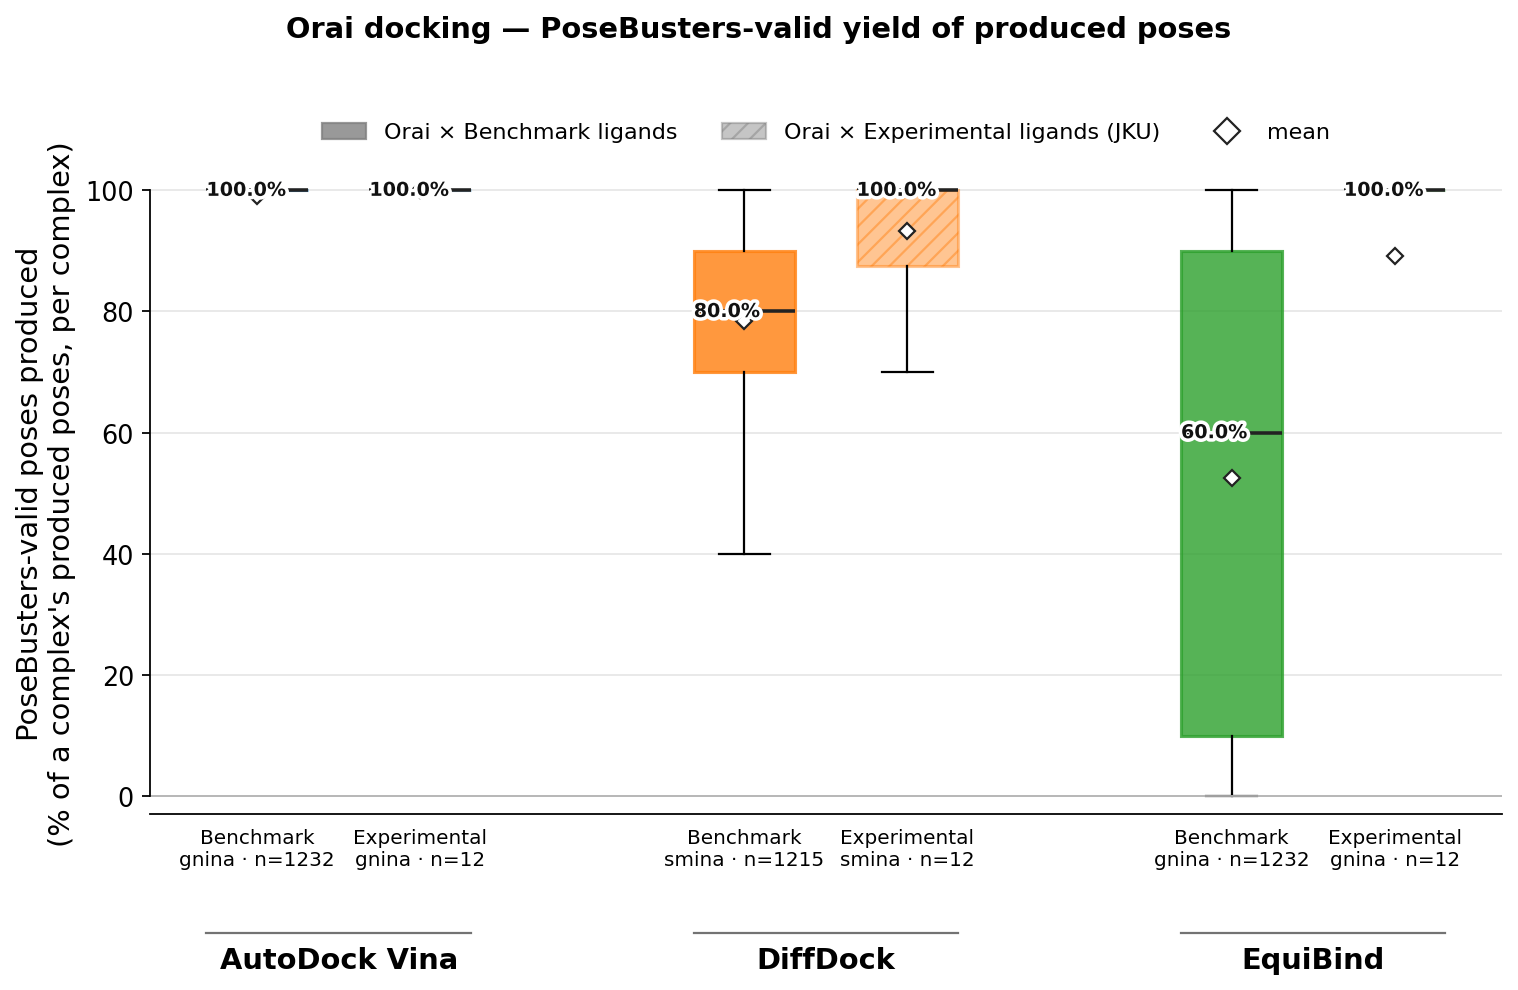
\includegraphics[width=\linewidth,height=0.78\textheight,keepaspectratio]{media/media/image13.png}
\caption{PoseBusters-valid yield of produced poses on Orai}\label{fig:results-r11}
\end{figure}

Figure~\ref{fig:results-r11} shows the smallest cross-panel change for AutoDock Vina. Median validity is 100\% in both panels, and the experimental mean is 100.0\% compared with 99.1\% in the benchmark. EquiBind changes most, from a benchmark median of 60\% and mean of 52.5\% to an experimental median of 100\% and mean of 89.2\%. DiffDock also improves, from a benchmark median of 80\% and mean of 78.5\% to an experimental median of 100\% and mean of 93.3\%. Fully valid units further distinguish the tools. Their benchmark rates are 97.0\% for AutoDock, 22.2\% for DiffDock and 22.9\% for EquiBind, rising to 100.0\%, 66.7\% and 83.3\% on the experimental ligands. EquiBind remains the most dispersed tool on the benchmark, where its lower quartile is 10\% and 19\% of units yield no valid pose.

The comparison of three experimental ligands with 308 controls has little power. Non-significance means that no difference was detected, not that none exists. Its cross-panel result therefore reflects ligand-set and pose-selection differences and remains descriptive. The physical-validity ordering is preserved in both Orai panels, consistent with but not proof of transfer from calibration.

\hypertarget{operational-placement-and-usable-yield}{%
\subsection{\texorpdfstring{Operational Placement and Usable Yield }{Operational Placement and Usable Yield }}\label{operational-placement-and-usable-yield}}

The operational placement rule defined in the Methods tests an outer-pore hypothesis. It does not replace a near-native endpoint or provide ground truth. Figure~\ref{fig:results-r12} in Appendix~\ref{orai1-panels} illustrates the rule on Fr300. The slab extends to the outer protein shell, consistent with the radially unbounded test rather than the narrower pore lumen.

Figure~\ref{fig:results-r13} reports per-unit usable yield in both panels.

\begin{figure}[!htbp]
\centering
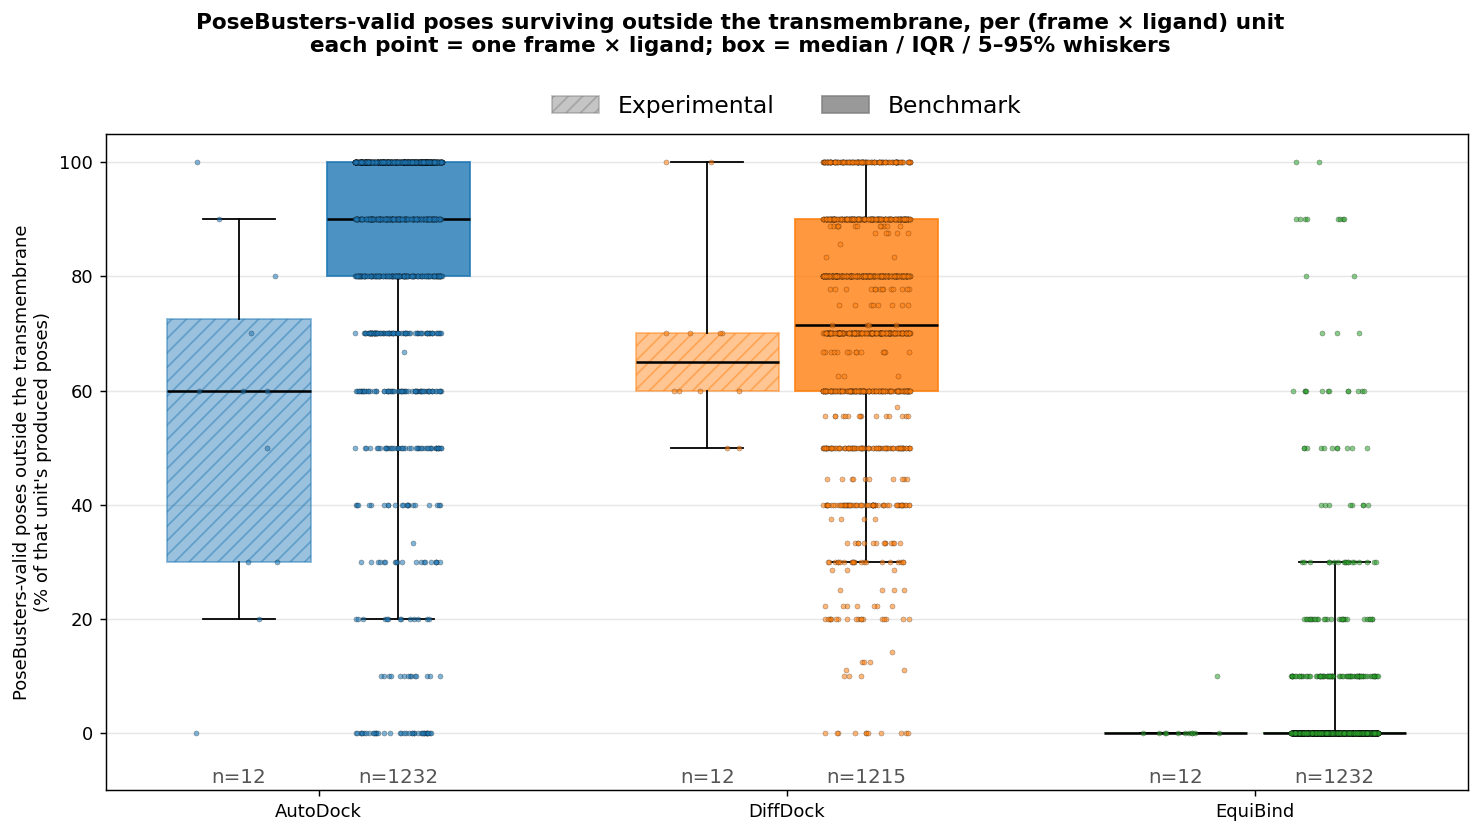
\includegraphics[width=\linewidth,height=0.78\textheight,keepaspectratio]{media/media/image43.png}
\caption{Usable pose yield per Orai frame-ligand unit}\label{fig:results-r13}
\end{figure}

AutoDock Vina leads on the benchmark but not the experimental ligands. Its medians are 90\% and 60\%, and its means 82.8\% and 54.2\%. DiffDock is lower on the benchmark (median 71.4\%) but higher experimentally (65.0\%), with means of 70.9\% and 68.3\%. EquiBind is degenerate in both panels. Its median and both quartiles are zero, with means of 3.8\% and 0.8\%.

An unpaired two-sided Mann-Whitney U test and Cliff\textquotesingle s \ensuremath{\delta}, where positive values favour the benchmark, compare frame-ligand units, removing pose nesting but not correlation among units from one ligand. AutoDock yields less experimentally than on the benchmark (U = 11749.0, \ensuremath{\delta} = +0.59, Holm p = 5.6e-4 across three tools). It is the only contrast that survives at both units and represents all three experimental ligands. The ligand-collapsed medians are 55.0\% and 92.5\% (\ensuremath{\delta} = +0.94, Holm p = 0.012). A panel-matching artefact inflates this contrast. Both panels retain ten poses, but the experimental ten are the gnina-best of thirty searched modes whereas the control ten are all that were written. Restricting the experimental panel to Vina modes one to ten moves the ligand-collapsed median from 55.0 to 70.0\% and its adjusted p from 0.012 to above 0.2, and the frame-ligand p from 5.6e-4 to 0.054 (Appendix~\ref{orai1-panels}). AutoDock still loses most between panels, but this adjusted significance does not survive matching. DiffDock trends in the same direction without significance (U = 8462.0, \ensuremath{\delta} = +0.16, p = 0.667), while EquiBind shows little change (\ensuremath{\delta} = +0.06, Holm p = 0.667).

The pooled pose-level analysis agrees but estimates rate differences rather than differences between per-unit means. These diverge for DiffDock because unit pose counts vary. AutoDock falls by 28.7 percentage points, from 82.83\% to 54.17\%, with a Fisher p below 1e-4 after correction, though the panel-matched restriction above puts that fall at 17.0 points. DiffDock changes by 2.7 points (71.07\% to 68.33\%) and EquiBind by 3.0 points (3.85\% to 0.83\%). Both are non-significant. With twelve correlated experimental units, these null results do not establish equivalence.

\begin{figure}[!htbp]
\centering
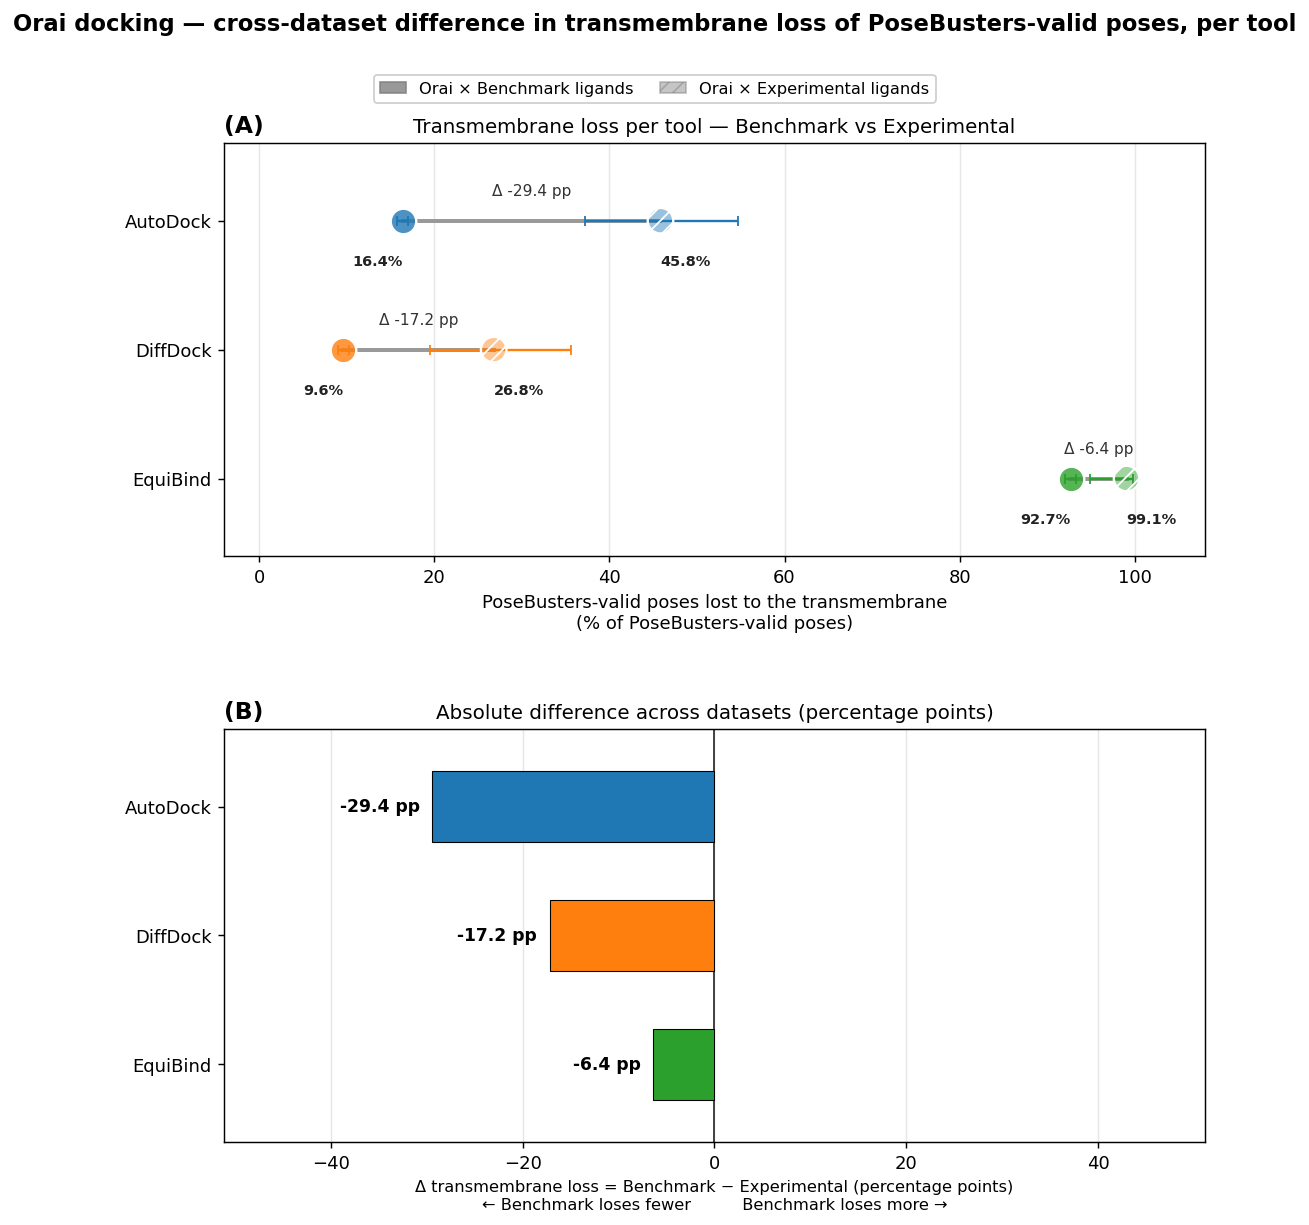
\includegraphics[width=\linewidth,height=0.78\textheight,keepaspectratio]{media/media/image15.png}
\caption{Transmembrane loss of PoseBusters-valid poses}\label{fig:results-r14}
\end{figure}

Figure~\ref{fig:results-r14} shows the proportion of PoseBusters-valid poses inside the slab under the same top-ten cap as Table~\ref{tab:results-orai-yield}. AutoDock Vina loses 16.4\% of control and 45.8\% of experimental poses, DiffDock 9.6\% and 26.8\%, and EquiBind 92.7\% and 99.1\%. These pose-level contrasts are descriptive because poses cluster within frame-ligand units. Together with Figure~\ref{fig:results-r13}, they distinguish validity from conditional placement. DiffDock loses less on both panels and therefore has higher experimental usable yield despite AutoDock Vina producing more valid poses. EquiBind almost entirely fails placement.

The per-unit usable-yield test corroborates only AutoDock Vina\textquotesingle s 29.4-point benchmark-to-experimental loss gap, at both the frame-ligand and ligand units. That gap is 17.8 points once the panels are matched on selection rule, so the corroboration is conditional on the caveat given above. The DiffDock and EquiBind gaps remain pooled descriptions. Absolute differences are preferable to ratios because the experimental denominator contains three ligands and at most twelve units, making the apparent 0.36-fold reduction in loss, which is 0.48-fold on the matched panels, unstable. Because the four frames sample one receptor, even the per-unit test is anti-conservative for generalisation to new ligands.

\hypertarget{cross-tool-clustering-1}{%
\subsection{Cross-Tool Clustering}\label{cross-tool-clustering-1}}

Clustering was performed for each MD frame, ligand and tool to assess cross-tool localisation and within-tool pose-cloud structure. Frames of one ligand are correlated snapshots of the same receptor-ligand system, so pooled medians are mildly pseudoreplicated. Collapsing each ligand across its frames gives a benchmark median of 29.3\angstrom{}, close to the pooled 28.4\angstrom{}. The experimental estimate changes from a pooled 38.1\angstrom{} to 40.3\angstrom{} after collapse and is therefore unstable, as expected from three ligands and eleven multi-tool units. Only the benchmark value is a stable central estimate.

\begin{figure}[!htbp]
\centering
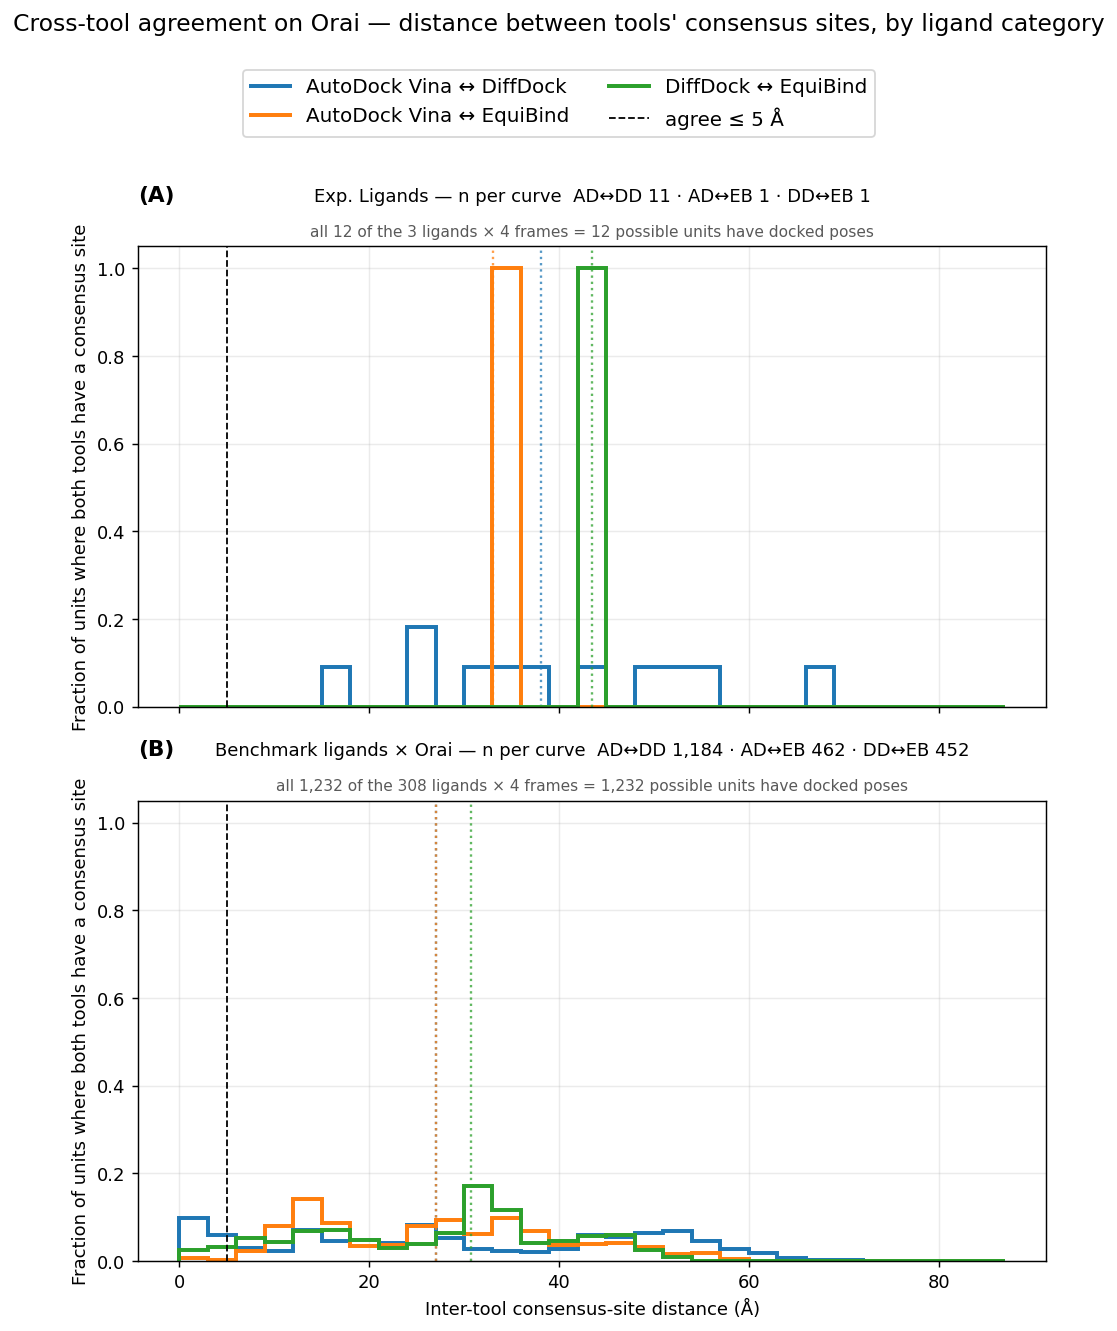
\includegraphics[width=\linewidth,height=0.78\textheight,keepaspectratio]{media/media/image16.png}
\caption{Distribution of inter-tool consensus-site distances on Orai. The dotted vertical lines mark the per-pair medians}\label{fig:results-r15}
\end{figure}

Figure~\ref{fig:results-r15} shows pairwise consensus-site distances. No experimental pair lies within the 5\angstrom{} threshold. Both benchmark EquiBind pairings are also sparse below it, whereas the tallest AutoDock--DiffDock bin lies just below 5\angstrom{}, despite most of that distribution lying above. Distances extend from a few ångströms to roughly 86\angstrom{} along the elongated pore. Pairwise medians are 27--31\angstrom{} for benchmark and 33--44\angstrom{} for experimental ligands. Continuous distances and pairwise rates are therefore more informative than the binary all-pairs flag, which requires every available pairing in a unit to lie within 5\angstrom{}. This occurs in 97 of 1,198 (8.1\%) multi-tool benchmark units and none of the eleven experimental units.

\begin{figure}[!htbp]
\centering

\includegraphics[width=\linewidth,height=0.78\textheight,keepaspectratio]{media/media/image17.png}
\caption{Cross-tool agreement on Orai}\label{fig:results-r16}
\end{figure}

Figure~\ref{fig:results-r16} resolves agreement by tool pair. For this endpoint, positive Cliff\textquotesingle s \ensuremath{\delta} means greater separation experimentally, opposite to the benchmark-higher orientation used for yield and cluster quality. The largest gap is DiffDock--EquiBind, at 43.5\angstrom{} experimentally versus 30.7\angstrom{} on the benchmark (\ensuremath{\delta} = +0.78). The contrast does not survive correction, and ligand-level collapse retains a single experimental ligand because neither Synta-66 nor GSK-7975A produced an EquiBind pose surviving the slab filter and top-ten cap. This is an exploratory estimate, not a corrected finding. The other two pairings are flat. AutoDock and DiffDock lie within 5\angstrom{} in 14\% of benchmark pairs but none of eleven usable experimental pairs. EquiBind pairings remain at or below 4\% on the benchmark and zero experimentally. Across all three pairings, 9\% of benchmark pairs and none of thirteen experimental pairs agree. Three-way agreement, which requires all three distances within 5\angstrom{}, occurs in two of 450 benchmark units with all three tools and not in the single experimental unit. AutoDock--DiffDock is therefore the only material agreement channel.

Reference-free cluster quality is reported in Figure~\ref{fig:results-r17} in Appendix~\ref{orai1-panels}, over six metrics on the raw pose cloud. DiffDock forms the tightest experimental clouds and EquiBind the loosest, often one diffuse mode. Only DiffDock\textquotesingle s Calinski-Harabasz index survives collapsing each ligand across four frames, and the appendix reads that as removal of within-ligand spread rather than new evidence.

Restricting benchmark clouds to PoseBusters-valid, outside-slab poses leaves within-cluster spread essentially unchanged for all three tools. Bootstrap stability rises significantly for all three, and DiffDock also improves on silhouette. Filtering increases reproducibility rather than tightness. Appendix~\ref{orai1-panels} gives the paired per-unit tests in Figure~\ref{fig:results-r18}, including the reduced EquiBind subset and degenerate single-cluster clouds that inflate its stability gain. Filtering does not detectably reduce the wide pore-axis scatter. Because no equivalence test was run, this bounds the observed filtering effect without establishing that the scatter is intrinsic to sampling.

AutoDock Vina forms the best-separated clouds and the tightest benchmark clouds, but precision without a reference does not establish accuracy. The broadly preserved ordering supports only cautious descriptive use of the control panel, not equivalence.

\protect\hypertarget{_Toc235735939}{}{}

\hypertarget{interaction-and-contact-analysis-1}{%
\subsection{Interaction and Contact Analysis}\label{interaction-and-contact-analysis-1}}

The analysis includes each tool\textquotesingle s top three PoseBusters-valid, outside-slab poses per frame-ligand unit. Both panels use the same four frames, making their residue axes directly comparable. PandaMap assigns residue-level contacts to fifteen interaction classes. After filtering, the experimental panel contains 32 poses from 11 AutoDock complexes and 36 from 12 DiffDock complexes, compared with 3,541 and 3,524 benchmark poses. EquiBind retains one experimental pose and 324 benchmark poses. Its results are non-interpretable and shown only for completeness. Figures display pose-level values, but significance tests first aggregate correlated poses to per-complex means. Contact-count and type-profile comparisons use unpaired Mann-Whitney U tests and Cliff\textquotesingle s \ensuremath{\delta}, with positive values favouring the benchmark.

Experimental poses have descriptively more contacts. The median rises from 27 to 30 for AutoDock Vina and from 15 to 18 for DiffDock. Neither difference survives per-complex testing, and collapsing each ligand across four frames leaves both untested, strengthening the AutoDock effect and weakening the DiffDock one. EquiBind\textquotesingle s single usable experimental pose is untestable and excluded from the correction family. No total-contact difference is detected at the available power, which does not establish equivalent contact intensity. Figure~\ref{fig:results-r19} in Appendix~\ref{orai1-panels} reports the distributions and four effect sizes.

\begin{figure}[!htbp]
\centering

\includegraphics[width=\linewidth,height=0.89\textheight,keepaspectratio]{media/media/image21.png}
\caption{Interaction-type profile on Orai}\label{fig:results-r20}
\end{figure}

Figure~\ref{fig:results-r20} reports mean interaction counts per pose. Alkyl-\ensuremath{\pi}, hydrophobic, other \ensuremath{\pi} and hydrogen-bond interactions dominate under both mature tools, but their order changes. Hydrogen bonds rank second on the benchmark and fifth experimentally. Benchmark ligands form more hydrogen bonds (Cliff\textquotesingle s \ensuremath{\delta} = +0.45 for AutoDock and +0.54 for DiffDock) and all ionic, salt-bridge and attractive-charge contacts. These charged classes are absent from both tools\textquotesingle s modulator poses. Modulators are more hydrophobic (\ensuremath{\delta} = \ensuremath{-}0.59 and \ensuremath{-}0.58) and richer in alkyl-\ensuremath{\pi} contacts (\ensuremath{-}0.42 and \ensuremath{-}0.59). They also register more halogen bonds, but that result carries no weight because the profiler is blind to chlorine and bromine and misses chlorine in part of the control library (Appendix~\ref{interaction-fingerprints}).

These patterns remain descriptive. At the frame-ligand unit, fourteen of twenty-six tool-by-type cells pass Benjamini-Hochberg correction. Two are the discounted halogen-bond cells, leaving twelve interpretable cells. None passes at the ligand unit, where the smallest adjusted values are 0.089 and 0.106. Table~\ref{tab:appendix-orai-interaction} gives the corresponding mean counts. The common direction is chemically plausible because the modulators are halogenated and lipophilic, whereas the benchmark library is more polar and hydrogen-bond driven, but it is not an established panel difference.

Both panels concentrate contacts on Asp110, Gln108, Tyr115, His113, Pro201 and Leu202. No residue differs after Holm correction of the fifteen within-tool tests. Figure~\ref{fig:results-r21} in Appendix~\ref{orai1-panels} gives the residue profiles.

\begin{figure}[!htbp]
\centering

\includegraphics[width=\linewidth,height=0.78\textheight,keepaspectratio]{media/media/image23.png}
\caption{Contact-fingerprint overlap between the two ligand sets}\label{fig:results-r22}
\end{figure}

Figure~\ref{fig:results-r22} compares contacted residues between panels. Residue-level Jaccard overlap is 0.42 for AutoDock and 0.31 for DiffDock, falling to typed-contact values of 0.40 and 0.27. Because all values use the same 10\% characteristic-contact threshold, these declines reflect changed interaction types rather than a changed basis. AutoDock shares 26 characteristic residues and DiffDock 13. EquiBind shares 5, but its overlap is uninterpretable from one experimental pose. The 10\% threshold also corresponds to roughly four experimental poses but several hundred benchmark poses. Diverse benchmark ligands distribute contacts broadly, whereas three repeatedly docked modulators concentrate them. The larger experimental-only count therefore reflects set size and homogeneity, not promiscuity. Shared residues and per-residue frequencies are more robust.

The surviving modulator poses partially agree with published pharmacology. Synta-66 maps to an extracellular TM1/TM3 region and adjoining loops near the E106 selectivity filter \cite{ref071}. Its defining extracellular loop1 and loop3 residues (His113, Tyr115, Pro201 and Leu202) lie above the filter and are characteristic of both tools\textquotesingle{} modulator poses. Leu109 is characteristic of both tools on the benchmark panel but of neither experimentally, at 9.4\% for AutoDock Vina and 5.6\% for DiffDock. Phe199 is characteristic of AutoDock Vina in both panels and of DiffDock only experimentally, where 19.4\% of poses contact it compared with 6.3\% on the benchmark. Each tool produces one modulator pose contacting Glu106, so neither consistently recovers the filter residue. These contacts support biological interpretation and hypotheses for mutagenesis or ligand-bound simulation, but evidence from different tools cannot be combined to validate one binding mode.

Net usable yield reverses the control-panel ordering. AutoDock Vina leads on controls, while DiffDock leads experimentally. Calibration point estimates show the same ordering, although not a statistically separable difference. EquiBind loses 106 of 107 valid poses to the exclusion rule and retains one of 120.

Three conclusions follow. First, physical validity alone overstates utility on a channel because a geometrically valid pose may occupy the ion-conduction pathway. Usable yield exposes EquiBind\textquotesingle s placement failures. Second, cross-tool consensus provides no reliable confidence signal. Median separation is roughly 30\angstrom{} on the benchmark and at least as large experimentally, although the experimental median is unstable after frame-robust collapse. At best 14\% of pairs agree within 5\angstrom{}. Symmetry folding is not applied to these separations. A rotation about the pore leaves the axial offset untouched and can shorten only the transverse part, so the six-fold symmetry of the channel cannot reconcile placements that differ along the pore. Appendix~\ref{orai1-panels} reports the separations without any symmetry correction. All three tools agree in two of 450 benchmark units and no experimental unit. Filtering valid, outside-slab poses does not detectably tighten the scatter, but without an equivalence test this only bounds the observed filtering effect.

Third, retained poses contain descriptive chemical signal. Both panels contact the same pocket residues, while modulators are more hydrophobic and less hydrogen-bonded, consistent with their halogenated lipophilic chemotypes. Both tools contact His113, Tyr115, Pro201 and Leu202. This does not conflict with large consensus-site distances. That metric uses each tool\textquotesingle s largest cluster, whereas residue sets pool all retained poses after six-fold symmetry folding. Arg170, Leu174 and Ala177 define an AutoDock-only sub-pocket below the Arg91 ring on the cytosolic face, associated with the Lys85 cluster. A further AutoDock cluster lies around Lys85 and neighbouring residues on the N-terminal segment below TM1. Neither cytosolic cluster supports the Synta-66 concordance. Both are reported for completeness.

Cross-panel agreement is limited. 19 of 54 testable contrasts have adjusted p below 0.05 at the frame-ligand unit and two at the ligand unit. The sensitivity analysis identifies one of the latter, DiffDock\textquotesingle s Calinski-Harabasz index, as a collapse artefact. AutoDock Vina\textquotesingle s lower experimental usable yield is the only result significant at both units and supported by all three ligands. It is the strongest cross-panel observation but remains descriptive, both because three ligands and four snapshots of one receptor cannot support general inference and because its adjusted significance does not survive matching the two panels on selection rule. For Orai1 the practical recommendation is therefore to retain AutoDock Vina and refined DiffDock as separate hypothesis generators, to prioritise poses that satisfy the validity and placement rules and agree with independent pharmacology, and to omit EquiBind in its present configuration. Sparse overlap between the two viable tools should not itself be treated as validation.

\hypertarget{pose-production-costs}{%
\section{Pose Production Costs}\label{pose-production-costs}}

Cost is normalised per qualifying pose, defined as PoseBusters-valid and within 2\angstrom{} of the crystal ligand. All docking used one workstation, whose specification and stage-specific devices are given in Appendix~\ref{docking-protocols}.

All figures use the whole-protein run of 303 complexes. The blind Vina search at exhaustiveness 128 took 4.73 wall-hours and gnina rescoring consumed 10.27 GPU-hours of device occupancy, making the rescorer roughly twice as expensive as the search it re-ranks. AutoDock therefore required 15.00 charged hours, 68.5\% for rescoring. Per-pose values divide this total.\footnote{Cost is charged as device occupancy throughout, on the single basis defined in the Methods: CPU-core-seconds divided by the 32 hardware threads of the workstation, plus GPU-seconds. Search and rescoring consume 151.42 CPU-core-hours and 10.27 GPU-hours. The CPU value is the search wall multiplied by 32 requested threads rather than measured occupancy, so dividing it by 32 returns the 4.73 wall-hours the search actually took and the charged total is that search time plus the rescorer's device occupancy. The rescoring pass was run sixteen ways concurrently and finished in 0.74 wall-hours, so its wall clock is a scheduling result rather than a property of the method. Charging it at wall clock instead would put AutoDock at 5.47 total wall-hours with 13.5\% for rescoring, and would flatter this arm against the pipelines it is compared with. The pass therefore summed roughly fourteen times its own wall clock across the sixteen workers, which changes elapsed time without changing the work done. Because neither CPU-core-seconds nor GPU-seconds are divided by that worker count, the charged basis is unaffected by it, whereas measured elapsed time is not.}

\begin{figure}[!htbp]
\centering

\includegraphics[width=\linewidth,height=0.78\textheight,keepaspectratio]{media/media/image24.png}
\caption[Charged seconds per qualifying pose]{Charged device-occupancy seconds per qualifying pose. Each box covers that pipeline's own 199, 169 and 80 qualifying complexes, while the bracketed tests use the 53 all three share}\label{fig:results-r23}
\end{figure}

\begin{longtable}[]{@{}
  >{\raggedright\arraybackslash}p{(\columnwidth - 12\tabcolsep) * \real{0.1600}}
  >{\raggedleft\arraybackslash}p{(\columnwidth - 12\tabcolsep) * \real{0.1400}}
  >{\raggedleft\arraybackslash}p{(\columnwidth - 12\tabcolsep) * \real{0.1700}}
  >{\raggedleft\arraybackslash}p{(\columnwidth - 12\tabcolsep) * \real{0.1200}}
  >{\raggedleft\arraybackslash}p{(\columnwidth - 12\tabcolsep) * \real{0.1500}}
  >{\raggedleft\arraybackslash}p{(\columnwidth - 12\tabcolsep) * \real{0.1200}}
  >{\raggedleft\arraybackslash}p{(\columnwidth - 12\tabcolsep) * \real{0.1400}}@{}}
\caption[Cost per Qualifying Pose]{Cost per Qualifying Pose. Charged medians and interquartile ranges are taken over the complexes for which that pipeline produced a qualifying pose. One basis applies to all four rows, namely CPU-core-seconds divided by the 32 hardware threads of the workstation plus GPU-seconds, so the charged column is directly comparable across pipelines. The CPU-core-second and GPU-second columns are pooled aggregates in their own currencies and are never summed}\label{tab:results-cost-per-qualifying-pose}\tabularnewline
\toprule\noalign{}
Pipeline & \shortstack[r]{Charged\\ median (s)\strut} & \shortstack[r]{Interquartile\\ range (s)\strut} & Complexes & \shortstack[r]{CPU-core-\\ seconds\strut} & \shortstack[r]{GPU-\\ seconds\strut} & \shortstack[r]{Qualifying\\ poses\strut} \\
\midrule\noalign{}
\endfirsthead
\toprule\noalign{}
Pipeline & \shortstack[r]{Charged\\ median (s)\strut} & \shortstack[r]{Interquartile\\ range (s)\strut} & Complexes & \shortstack[r]{CPU-core-\\ seconds\strut} & \shortstack[r]{GPU-\\ seconds\strut} & \shortstack[r]{Qualifying\\ poses\strut} \\
\midrule\noalign{}
\endhead
\bottomrule\noalign{}
\endlastfoot
AutoDock & 137.2 & 75.6 to 167.4 & 199 & 1,752.8 & 118.9 & 311 \\
DiffDock & 49.4 & 14.1 to 127.3 & 169 & 2.93 & 49.9 & 1,622 \\
EquiBind & 2.4 & 1.0 to 7.3 & 80 & 165.3 & 1.4 & 466 \\
\midrule\noalign{}
AutoDock, Vina search only & 21.7 & 9.9 to 45.3 & 202 & 1,805.0 & 0.0 & 302 \\
\end{longtable}

The configured AutoDock pipeline is the most expensive route to a qualifying pose under blind whole-protein search. Figure~\ref{fig:results-r23} shows the per-complex charged distributions, and Table~\ref{tab:results-cost-per-qualifying-pose} reports all three currencies. Among 53 complexes where every tool succeeds, the ordering persists (Friedman \ensuremath{\chi}\textsuperscript{2} = 85.2, p = 3.2e-19, Kendall W = 0.80), and every pair passes Holm correction. Median per-complex cost ratios are 0.14 for DiffDock versus AutoDock and 0.02 for EquiBind. gnina raises AutoDock cost to roughly three times the search alone, then that total is amortised over few qualifying poses. The median successful complex yields one, although 199 of 303 complexes now yield at least one, far more than the 169 of DiffDock.

Tightening the endpoint increases cost most for AutoDock. Median charged seconds per generated, valid, and valid-near-native pose are 5.3, 5.3 and 137.2 for AutoDock. The DiffDock values are 7.6, 9.2 and 49.4, and the EquiBind values are 0.3, 0.4 and 2.4. Contributing complexes fall from 303 to 301 to 199 for AutoDock, 303 to 300 to 169 for DiffDock, and 303 to 266 to 80 for EquiBind. Moving from valid to valid-near-native multiplies unit cost by about 25.9, compared with 5.4 for DiffDock and 6.0 for EquiBind. The multiplier is large for AutoDock because a complex that succeeds contributes only one or two qualifying poses out of thirty, not because it succeeds rarely. EquiBind\textquotesingle s 2.4 s median describes only the 80 successful complexes. It fails in the other 223.

\begin{figure}[!htbp]
\centering

\includegraphics[width=\linewidth,height=0.78\textheight,keepaspectratio]{media/media/image25.png}
\caption{Hardware resource per qualifying pose. The two currencies are pooled aggregates and are never summed}\label{fig:results-r24}
\end{figure}

Removing parallelism from the resource axis widens the separation (Figure~\ref{fig:results-r24} and Table~\ref{tab:results-cost-per-qualifying-pose}). Configured AutoDock is most expensive on every axis. Its 32 threads compress 151.42 CPU-core-hours of search into 4.73 wall-hours. The subsequent GPU rescoring pass adds device occupancy without adding CPU cost. The tools convert their compute into 311, 1,622 and 466 qualifying poses, which explains much of the gap. GPU time covers docking for DiffDock and EquiBind but only gnina rescoring for AutoDock. AutoDock nevertheless has the highest GPU cost per qualifying pose because its qualifying yield is low.

Four caveats apply. First, wall-clock time is cross-hardware and device mixes differ within and between pipelines. AutoDock spends 4.73 of its 15.00 charged hours on a multithreaded CPU and 10.27 on a GPU shared by up to sixteen concurrent workers, so elapsed time does not measure identical work. Second, resource values are order-of-magnitude estimates. AutoDock CPU-core-seconds cover only Vina and assume all 32 threads are occupied, while gnina is recorded separately as GPU occupancy. Third, part of the AutoDock rescoring pass is an implementation artefact. The rescorer was invoked once per pose, and each invocation paid the start-up of a separate process on a GPU that a single-pose evaluation leaves substantially idle. Batching would therefore reduce the cost of the learned rescorer by an amount this run does not determine. Fourth, the charged basis credits every pipeline with full use of the 32 threads, which the three arms did not realise equally. Vina already occupies all 32 within a single docking, whereas EquiBind reaches that occupancy only by running separate complexes concurrently, so its charged figure is an idealised best-configuration estimate rather than a measured elapsed time. Its 21.39 CPU-core-hours are under a seventh of AutoDock\textquotesingle s 151.42. The uniform basis therefore makes the three columns arithmetically comparable without making the underlying concurrency equally attainable, and EquiBind\textquotesingle s figure should be read as a floor. The pooled resource panel has no inferential test, but pipeline success differs strongly at the complex level (Cochran\textquotesingle s Q = 61.1, p = 5.5\ensuremath{\times}10\textsuperscript{\ensuremath{-}14}).

Under the blind whole-protein configuration used throughout this chapter, configured AutoDock is most expensive per qualifying pose in charged, CPU and GPU terms. This does not apply to the classical search alone. Without gnina, Vina requires a median 21.7 s and no GPU time per qualifying pose, still below DiffDock on the charged basis. Its CPU cost per qualifying pose is 1,805.0 s, higher than the rescored arm\textquotesingle s 1,752.8 s, because rescoring adds nine qualifying poses at no CPU cost. Vina remains by far the most processor-intensive engine on either arm, while AutoDock becomes most expensive in charged and GPU time only after learned rescoring. It is also not cheapest per generated pose on any currency (Table~\ref{tab:appendix-cost-per-pose}). Its advantage is coverage and admissibility, not economy.

The ordering depends on the denominator rather than on the currency. Median charged time per attempted docking is 157.7 s for AutoDock, 227.6 s for DiffDock and 8.1 s for EquiBind. Because each produces about thirty poses per complex, this rescales the per-complex median rather than providing an independent measure. Allocating the whole campaign to complexes that yield a qualifying pose gives 271, 479 and 38 s. On this denominator AutoDock is cheaper than DiffDock in charged and GPU terms, with 186 versus 478 GPU-seconds per success, but remains much more expensive in CPU-core-seconds. Neither denominator changes the per-qualifying-pose result.

\hypertarget{discussion}{%
\chapter{\texorpdfstring{Discussion }{Discussion }}\label{discussion}}

\hypertarget{principal-findings-and-scope-of-inference}{%
\section{Principal Findings and Scope of Inference}\label{principal-findings-and-scope-of-inference}}

This study compared AutoDock Vina, DiffDock and EquiBind by crystallographic re-docking of 303 calibration complexes and reference-free docking of three Orai1 modulators into four molecular-dynamics snapshots. The calibration benchmark provides stronger evidence because each prediction has an experimental reference. Its endpoints favour AutoDock without settling the comparison. Under the blind whole-protein search, AutoDock had the highest physical validity and led DiffDock on near-native recovery and native-pocket reach at every depth. The near-native lead is inconclusive at rank-1 and separable from top-5 onwards, and reach never separated them. The rank-1 interval spans a 4.2-point DiffDock lead to a 9.4-point AutoDock lead. Refined EquiBind had low raw validity, in-place accuracy and pocket localisation. Orai1 preserved the validity ordering but reversed the usable-yield ordering. Without a ligand-bound structure, neither result identifies the correct binding mode.

These findings rank the configured pipelines, not artificial intelligence and physics as method classes. Newer diffusion, co-folding and hybrid systems report gains from specified pockets, receptor flexibility and structural relaxation \cite{ref012}, \cite{ref031}, \cite{ref064}, \cite{ref069}. Similarity-controlled and perturbation analyses also show that aggregate accuracy can conceal reliance on training-set analogues and weak extrapolation to new pockets \cite{ref035}, \cite{ref063}, \cite{ref065}, \cite{ref069}. This thesis therefore contributes a separation of sampling, ranking, validity and localisation failures rather than a permanent method ranking.

Physics-based is itself an operational label here. Vina combines explicit search with an empirical score. It is not a molecular-mechanics or free-energy simulation. Its result supports the evaluated classical search-and-score workflow, not a complete physical model of binding.

\hypertarget{physical-validity-and-post-docking-optimisation}{%
\section{Physical Validity and Post-Docking Optimisation}\label{physical-validity-and-post-docking-optimisation}}

The largest initial separation preceded RMSD assessment. Under the blind whole-protein configuration used here, pooled validity differed by more than seventy percentage points between AutoDock Vina and the raw learned outputs. Local optimisation then made many learned poses admissible. This margin is partly constitutive because the discriminating intermolecular checks inspect coordinates already minimised by Vina, as Appendix~\ref{validity-objective-coupling} explains. Its effect on the headline endpoint is small, however. Requiring validity removes at most four of 303 complexes at any depth. RMSD alone is therefore insufficient, since a geometrically close ligand can still have unrealistic bonds, steric overlap or intermolecular contacts \cite{ref035}. Combined accuracy and validity are more discriminating \cite{ref013}, \cite{ref032}.

Local optimisation mainly repaired geometry, not blind placement. DiffDock validity rose sharply while its fixed-rank near-native rate barely changed. EquiBind showed a modest near-native increase. Table~\ref{tab:appendix-refinement-bands} reports these changes by rank band.

Refiner selection remains an empirical pipeline choice, and the two families behave differently. For DiffDock the refiners are interchangeable. smina is carried forward on the selection criterion by 133 complexes to 132, but that one-complex margin survives only in the three-way conjunction of validity, near-nativeness and form. Dropping either the validity or the form term leaves the two arms exactly level, and gnina is level or ahead on every component taken alone. Exact McNemar separates them at no depth. For unguided EquiBind the choice is not immaterial. gnina recovers 83 near-native complexes at top-15 against 61 for smina, and that difference survives Holm correction. Only on the selection endpoint, where the margin is nine complexes, are the two EquiBind arms not separable. The study measured neither optimisation trajectories nor refiner performance on an independent set, so proposed mechanisms such as gentle preservation or aggressive repair remain interpretations.

PoseBusters validity is not binding stability. Passing Table~\ref{tab:appendix-posebusters-checks} excludes important chemical, conformational and steric failures but establishes neither favourable binding free energy, correct protonation or tautomer states, water or ion mediation, nor persistence in a membrane. Validity is an admissibility filter. Placement, interaction recovery and prospective experiments test accuracy separately.

\hypertarget{sampling-ranking-and-interaction-recovery}{%
\section{Sampling, Ranking and Interaction Recovery}\label{sampling-ranking-and-interaction-recovery}}

Ranking depth separates generation from selection. Moving from rank-1 to the best of fifteen substantially increased recovery for DiffDock and AutoDock but added only about eight percentage points for EquiBind (Results, Near-Nativeness and Form). Useful DiffDock and AutoDock poses were therefore often under-ranked. Selection was not the main loss. About six in ten rank-1 failures of the two tools contained no qualifying pose at any depth. The corresponding share for EquiBind was about nine in ten. Re-ranking cannot recover an absent binding mode.

The form decomposition supports this result. AutoDock and DiffDock were indistinguishable on internal form at the prespecified 1\angstrom{} Kabsch threshold, while AutoDock led on near-nativeness from top-5 onwards. DiffDock often generated a credible conformation without ranking it first. EquiBind was weaker on both axes. A ligand can retain its shape while presenting its pharmacophore to the wrong residues, so form and placement must remain distinct.

Pocket recovery was easier than exact pose recovery under the whole-protein search. AutoDock and DiffDock intervals overlapped throughout. AutoDock had the higher point estimate at top-15, but the paired reach test in the calibration Cross-Tool Clustering section did not separate them. Pooling all tools placed the crystal pocket somewhere in the pose cloud for 95\% of complexes, but the best inexpensive cluster rule ranked it first in only 57\%. This is a site-selection gap, not 95\% exact-pose accuracy. Cluster membership is coarser than a valid pose within 2\angstrom{}.

Interaction fingerprints show the same dependence on endpoint and depth. DiffDock had the highest mean crystal overlap for the union of top-five contacts, but the leading tools were not separable at rank-1. This is inconclusive rather than equivalent. The one equivalence statement in this work covers the valid-near-native recovery contrast, and its margin was read off the data after the fact rather than prespecified. AutoDock contact recovery declined through its top five while DiffDock remained flat, yet DiffDock confidence was not detectably associated with interaction recovery. AutoDock therefore ranked a weaker pool more effectively, and EquiBind missed more native contacts than it recovered at every rank. External scores require validation for their intended task \cite{ref067}.

\hypertarget{generalisation-in-the-context-of-current-literature}{%
\section{Generalisation in the Context of Current Literature}\label{generalisation-in-the-context-of-current-literature}}

The benchmark\textquotesingle s post-2021 construction reduces temporal overlap with early training data but cannot exclude homologous receptors, familiar pockets or related ligands. PoseBusters performance declined at low receptor sequence identity \cite{ref035}, and Li et al. identified pocket novelty as a central generalisation constraint \cite{ref013}. On the PDBbind time split, the TEMPL baseline rose from 22.1\% overall to 67.3\% when related protein and ligand templates were available, then collapsed outside that region \cite{ref065}. Time alone therefore does not establish novelty.

PoseBench likewise found that modern co-folding systems outperformed several conventional and learned baselines overall but remained challenged by new binding poses and the joint demands of structural accuracy and chemical specificity \cite{ref069}. PoseX reported gains from recent AI and co-folding systems after relaxation and from pocket information and physics-inspired post-processing \cite{ref012}. Performance therefore depends on model generation, benchmark novelty, receptor information, flexibility and relaxation. EquiBind\textquotesingle s result is consistent with early one-shot models trailing newer systems. The DiffDock result identifies limits of this version\textquotesingle s blind placement, validity and confidence ranking, not a ceiling on generative docking.

\hypertarget{interpretation-of-the-reference-free-orai1-study}{%
\section{Interpretation of the Reference-Free Orai1 Study}\label{interpretation-of-the-reference-free-orai1-study}}

Orai1 is more realistic but less identifiable than crystallographic re-docking. AutoDock Vina produced valid poses for all three modulators but retained a smaller share after the combined on-receptor and transmembrane-placement screen. Refined DiffDock had lower validity but more usable poses. That ordering depends on the ranking each pipeline applies before the cap, since the gnina re-ranking that improves AutoDock rank-1 recovery on the crystal benchmark selects against the placement rule here, and reverting AutoDock to its Vina order restores it to the higher yield. EquiBind retained one of 120. Without an experimental ligand pose, these rates measure admissibility rather than near-nativeness.

The R91--E106 exclusion slab encodes an outer-pore hypothesis. GSK-7975A sensitivity has been linked to filter geometry through a proposed allosteric effect rather than direct pore block \cite{ref070}, while Synta-66 has been mapped to an extracellular TM1/TM3 and loop region \cite{ref071}. Excluding the conduction pathway is therefore defensible but not ground truth. The result establishes only that EquiBind produced almost no valid, on-receptor poses outside this study\textquotesingle s slab.

Cross-tool disagreement compounds this uncertainty. AutoDock Vina and DiffDock agreed within 5\angstrom{} in none of eleven evaluable experimental pairs, compared with 14\% of control pairs, and no experimental unit had three-way consensus. The experimental distance median was unstable under frame-robust collapse, so equal scatter between panels cannot be inferred. AutoDock formed better-separated clouds and DiffDock tighter ones, but compactness measures precision, not accuracy. Recovery of literature-associated filter and TM1/TM3 residues therefore generates hypotheses. Neither partial contacts nor their combination validates a complete pose.

At the ligand unit, only AutoDock Vina\textquotesingle s lower usable yield on the modulators survived the experimental-versus-control analysis, and that survival is itself conditional on the two panels being capped by different selection rules (Appendix~\ref{orai1-panels}). Other placement, clustering and interaction contrasts either lost corrected significance or rested on one or two ligands. Three chemotypes, four correlated frames and almost no EquiBind output give little power to establish either differences or equivalence. Physical-validity ordering transferred across panels, whereas usable-yield ordering reversed, so the control panel supports only cautious reference-free comparison. A stronger study would add independent trajectories, systematic frame selection, explicit membrane and ion conditions, ligand-bound simulations and experimental mutagenesis or competition assays. The experimental work lies outside this thesis and continues at Johannes Kepler University Linz (JKU).

\hypertarget{computational-efficiency-and-practical-tool-selection}{%
\section{Computational Efficiency and Practical Tool Selection}\label{computational-efficiency-and-practical-tool-selection}}

Within the whole-protein configuration, EquiBind had the shortest median charged cost per qualifying pose, followed by DiffDock and AutoDock. All three are charged on one basis, device occupancy on a 32-thread processor and a single GPU, so the ordering is a comparison of like with like. What differs is how attainable each pipeline's concurrency is, since EquiBind reaches full thread occupancy only across separate complexes, and how many complexes each ordering rests on, EquiBind succeeding on 80 of 303 against 169 for DiffDock. The ordering is therefore firmer than its magnitude. Within this protocol, configured AutoDock was the most expensive route on the charged and hardware axes. Its return was coverage and validity rather than speed.

Hybrid evidence supports this interpretation. DiffDock-Glide improves sampling through pocket-conditioned diffusion and physics-based minimisation \cite{ref064}, PoseX reports that relaxation removes many AI steric failures \cite{ref012}, gnina 1.3 improves ranking within a classical sampler \cite{ref067}, and CACHE produced experimental hits with an open hybrid workflow without establishing universal superiority \cite{ref068}. Learned generation is most useful when paired with physical validation and task-specific ranking.

\hypertarget{implications-for-docking-workflows}{%
\section{Implications for Docking Workflows}\label{implications-for-docking-workflows}}

The results support a staged workflow that generates several hypotheses, optimises local geometry, rejects invalid or biologically inadmissible structures, ranks the remainder with an endpoint-specific selector and retains uncertainty when tools disagree. Refined DiffDock and AutoDock Vina are complementary. AutoDock has higher accuracy and pocket-localisation point estimates, while DiffDock costs less per qualifying pose. Their rank-1 near-nativeness gap is unresolved. EquiBind provides too little coverage for routine use in this configuration. Its Orai1 control panel yielded only 3.8\% usable poses, compared with 82.8\% for AutoDock and 71.1\% for DiffDock.

Future comparisons should match information and compute across current flexible diffusion and packing methods \cite{ref031}, multi-pocket conditioning \cite{ref066}, hybrid refinement \cite{ref064}, co-folding systems \cite{ref012}, \cite{ref069} and template controls \cite{ref065}, using protein-, pocket- and ligand-novel splits. EquiBind was worse with an fpocket- or P2Rank-predicted pocket than without one (Appendix~\ref{equibind-pocket-guided}), which shows that pocket detection helps only if the docking model uses it effectively. Blind community evaluation can combine flexibility-aware, hybrid and leakage-controlled testing \cite{ref047} while keeping benchmark accuracy distinct from reference-free biological hypotheses.

\hypertarget{conclusions}{%
\chapter{\texorpdfstring{Conclusions }{Conclusions }}\label{conclusions}}

\hypertarget{rq1-quality-and-stability}{%
\section{RQ1: Validity, Near-Nativeness and Ranking Depth}\label{rq1-quality-and-stability}}

All pipelines searched the whole receptor, and the headline metric required PoseBusters validity and an RMSD within 2\angstrom{}. Rank-1 recovery was 36.6\% for AutoDock, 34.0\% for DiffDock and 18.2\% for EquiBind. Retrospective top-15 recovery was 65.3\%, 55.1\% and 26.4\%. The AutoDock--DiffDock rank-1 difference was +2.6 percentage points (95\% interval \ensuremath{-}4.2 to +9.4) and was not statistically resolved, although AutoDock led from top-5 onwards, by +13.2 points there (p\_holm = 7.6e-4) and +10.2 at top-15. That ordering is conditional on search effort. AutoDock ran at exhaustiveness 128, the top rung of a five-value ladder, and no measurement here speaks to what a harder search would return (Appendix~\ref{exhaustiveness-selection}). A post-hoc 90\% compatibility interval places the rank-1 difference within about eight points. It is descriptive, not a prespecified equivalence test. Both leading tools remained decisively ahead of EquiBind.

Physical validity separated the tools in the same order, at 98.9\%, 84.5\% and 62.0\%, although part of this separation is constitutive (Appendix~\ref{validity-objective-coupling}). Rank-1 native-interaction recovery likewise did not separate the leading tools. DiffDock led only for the top-five contact union. On Orai1, median usable yield under the study\textquotesingle s placement rule was 65\% for DiffDock, 60\% for AutoDock and 0\% for EquiBind. This untested reversal rests on twelve correlated units from three ligands and is descriptive. It is also conditional on the ranking cap each pipeline carries. AutoDock is capped on its gnina re-ranking, and restricting it instead to Vina modes one to ten puts it at 75\% and removes the reversal, whereas the DiffDock cap is close to neutral on this endpoint. The five-point deficit is therefore a property of the secondary ranker rather than of the search. Only one of 120 EquiBind poses passed both screens. The separate control panel put AutoDock first.

These endpoints measure static geometry, physical validity and pose placement. None of them tests thermodynamic or time-dependent stability.

\hypertarget{rq2-effect-of-post-docking-optimisation}{%
\section{RQ2: Effect of Post-Docking Optimisation}\label{rq2-effect-of-post-docking-optimisation}}

Local optimisation mainly repaired geometry. DiffDock validity rose from 24.4\% raw to 84.5\% with smina and 87.1\% with gnina. EquiBind rose from 2.9\% to 51.3\% and 62.0\%. Fixed-rank near-native rates changed by only 0.1--0.7 percentage points for DiffDock, 4.1--4.6 for EquiBind with gnina and 3.5--4.4 with smina. The larger top-\emph{k} gains in Table~\ref{tab:appendix-refinement-mcnemar} accumulate them across ranks, and gnina also re-ranks EquiBind poses. AutoDock gained by re-ranking, from 31.0\% to 36.6\% at rank-1. That single step does not clear Holm correction on its own, and the gain reaches significance only from top-5 onwards. Optimisation therefore made many learned poses admissible but could not supply a binding mode or fix gross placement.

\hypertarget{rq3-computational-efficiency}{%
\section{RQ3: Computational Cost and Accounting Basis}\label{rq3-computational-efficiency}}

Across 303 whole-protein searches, median charged cost per qualifying pose was 2.4 s for EquiBind, 49.4 s for DiffDock and 137.2 s for AutoDock. DiffDock succeeded on 169 complexes, AutoDock on 199 and EquiBind on 80. All three are charged on one basis, CPU-core-seconds divided by the 32 hardware threads of the workstation plus GPU-seconds, so the figures are comparable in basis as well as in scope. Every tool is charged for the configuration carried forward and for nothing else. AutoDock Vina and DiffDock each produced a single configuration, and for them the charged cost and the whole run are the same number. EquiBind produced nine configurations in one pass, of which only the unguided gnina configuration is reported. The remaining twentyfold EquiBind advantage over DiffDock is therefore a property of the work performed rather than of the accounting, though it is conditional on EquiBind succeeding on a quarter of the set and on a thread occupancy it reaches only across separate complexes.

Configured AutoDock was most expensive per qualifying pose in charged, CPU-core and GPU seconds. This does not apply to Vina alone. Removing gnina puts its charged and GPU cost below DiffDock, although Vina retains the highest CPU-core cost. The 4.73-hour blind search and 10.27-hour gnina pass total 15.00 charged hours, 68.5\% of which belongs to rescoring. Per-pose process start-up leaves the GPU underused, so batching should reduce this cost by an unmeasured amount. These results describe the implementations and hardware, not method classes.

\hypertarget{rq4-opportunities-and-limitations}{%
\section{RQ4: Opportunities and Limitations}\label{rq4-opportunities-and-limitations}}

The tools fail differently, which favours a staged workflow of generating candidates, optimising geometry, screening validity and placement, then ranking with an endpoint-specific selector. The evidence remains limited to single configured settings without multi-seed sweeps, a post-2021 benchmark that cannot exclude similarity leakage, and three Orai1 chemotypes across four correlated frames without a cognate structure.

AutoDock had the highest PoseBusters pass rate and in-place point estimates, but near-nativeness separated it from DiffDock only from top-5 onwards. Generation and localisation dominated failure. About six in ten AutoDock and DiffDock rank-1 failures, and nine in ten EquiBind failures, contained no qualifying pose. Selection still recovered 87 and 64 additional complexes at top-15 for the leading tools, compared with 25 for EquiBind. The result is a workflow, not a universal winner.

\hypertarget{limitations-and-future-outlook}{%
\chapter{Limitations and Future Outlook}\label{limitations-and-future-outlook}}

No method dominates under the pocket-free conditions tested here. AutoDock Vina remains limited by a rigid receptor and empirical score, so the staged hybrid workflow requires independent validation of its final hypotheses.

DiffDock stochasticity limits reproducibility. The 303-complex calibration run is one unseeded draw made before the local seed patch. Rerunning it may change the pose sample. The Orai1 experimental panel uses seed 42 and is repeatable under the recorded environment, although bitwise determinism was not tested. The unseeded Orai1 control panel supplies most reported Orai DiffDock values (Table~\ref{tab:appendix-orai-protocols}). No arm was assessed across multiple seeds.

Variant selection and evaluation use the same 303 complexes, with no held-out split. On the variant-selection endpoint at the top-15 depth at which the choice was made, the winning margins were eight complexes for AutoDock Vina, one for DiffDock and nine for EquiBind. Only the AutoDock margin is separable, and it is the one drawn from the largest field, the eight configurations of Table~\ref{tab:appendix-exhaustiveness-ladder} against three refiner arms for each learned pipeline. The largest of those margins is 3.0 percentage points of the 303, which bounds the optimism the selection can have introduced in any one family. A winner\textquotesingle s-curse correction computed per family over three arms puts it between 0.4 and 0.8 percentage points, and Appendix~\ref{exhaustiveness-selection} gives the larger correction that the eight-arm AutoDock field carries. EquiBind also confounds geometry with ranking because gnina performs both, whereas DiffDock refinement preserves rank. All three refined arms were run in the same energy-minimisation mode (\texttt{-{}-minimize}), so the calibration-benchmark validity figures are a like-for-like comparison (Appendix~\ref{docking-protocols}).

Further limits concern denominators and endpoints. Two corrected DiffDock defects are documented in Appendix~\ref{orai1-panels}. The Orai control cap was ten rather than thirty poses and was not reached in 178 of 1,215 units. Post-2021 release does not exclude leakage, and blind whole-protein AutoDock results are not comparable with published site-centred cognate re-docking. The two arms also differ on the receptor axis. Every calibration complex is re-docked into its own cognate crystal receptor, whereas the Orai1 arm docks into non-cognate molecular-dynamics snapshots of a homology model, and cognate self-docking is the easier of the two regimes, so the calibration figures bound the Orai1 expectation from above rather than predicting it. Receptor preparation also removed waters, ions, metals and cofactors for the AutoDock and DiffDock arms. A metal ion or metal-containing cofactor lies within 5\angstrom{} of the crystal ligand in 78 of the 303 calibration complexes, so recovery across that quarter of the set is measured without a coordinating partner the crystal pose depends on. The AutoDock-over-DiffDock top-15 contrast is +6.7 percentage points on the 225 metal-free complexes against +20.5 on the 78 metal-adjacent ones, so the pooled contrast averages a narrow gap with a much wider one (Appendix~\ref{autodock-vina-2}). Poses within a complex and four frames from one receptor are correlated, making the complex or trajectory the inferential unit. Best-of-top-\emph{k} and crystal-nearest clusters are oracle ceilings rather than prospective rank-1 accuracy.

PoseBusters tests gross geometry, not binding stability, and no ligand-bound dynamics were run. No endpoint reported here resolves binding free energy. Recovery, physical validity and RMSD are geometric criteria, and no score used for ranking was compared against measured affinities. Its internal-energy check depends on pose-file hydrogens, preventing direct comparison of raw and optimiser-written arms on that check. The interaction profiler misses chlorine and bromine in its halogen test and records each charged contact in three classes. Appendix~\ref{interaction-fingerprints} therefore treats those classes as one measurement. The Orai1 slab is a uniform operational hypothesis despite ligand-specific pharmacology and may exclude valid GSK-7975A or Synta-66 poses \cite{ref070}, \cite{ref071}. Cost per qualifying pose is conditional on success and therefore favours EquiBind.

AutoDock Vina requires a search box, whereas DiffDock and EquiBind localise the ligand. Equalising information therefore withheld site information from Vina. This whole-protein box is stricter than blind benchmarks that supply predicted pockets, such as PoseBench\textquotesingle s P2Rank--Vina arm \cite{ref069}, \cite{ref061}, but matches pocket-free DiffDock baselines \cite{ref024}, \cite{ref091}. The validity advantage persists under this design, although search, scoring and local optimisation remain inseparable.

A predicted-pocket Vina arm would provide an intermediate comparison. Under-sampling and blind search were separated only along the sampling axis, since no predicted-pocket Vina arm was run. Appendix~\ref{search-effort-and-box-volume} gives the box distribution and the convergence evidence, and Appendix~\ref{exhaustiveness-selection} what raising the search effort recovered.

The Orai1 poses remain computational hypotheses. Validation requires site-directed mutagenesis, competition or displacement assays and ideally a ligand-bound structure. This work continues at JKU. The reference-free arm contributes a documented, physically screened workflow for testable hypotheses, not a validated complex.
